% Created 2024-04-30 Tue 15:08
% Intended LaTeX compiler: pdflatex
\documentclass[aspectratio=169]{beamer}
\usepackage[utf8]{inputenc}
\usepackage[T1]{fontenc}
\usepackage{graphicx}
\usepackage{longtable}
\usepackage{wrapfig}
\usepackage{rotating}
\usepackage[normalem]{ulem}
\usepackage{amsmath}
\usepackage{amssymb}
\usepackage{capt-of}
\usepackage{hyperref}
\logo{
\includegraphics[height=0.5cm]{img/u-state-black.png}}
\usepackage[ruled]{algorithm2e}             % Algorithms
\usepackage{tikz}                           % Draw stuff
\usetikzlibrary{arrows.meta}                % Arrows for tikz
\institute[USU] % (optional)
{
College of Engineering\\
Utah State University
}
\addtobeamertemplate{navigation symbols}{}{%
\usebeamerfont{footline}%
\usebeamercolor[fg]{footline}%
\hspace{1em}%
\insertframenumber/\inserttotalframenumber
}
\AtBeginSection[]
{
\begin{frame}
\frametitle{Table of Contents}
\tableofcontents[currentsection]
\end{frame}
}
\newcommand\mycommfont[1]{\footnotesize\ttfamily\textcolor{gray}{#1}}
\newcommand{\T}{\mathcal{T}}                % To make it clear the difference
\newcommand{\Tau}{T}                        % between Tau and T
\newcommand{\AC}{AC(u, d, v, \eta)}         % Set the parameters for AC once
\newcommand{\UC}{UC(u, d, v)}               % Set the parameters for UC once
\newcommand{\ACi}{AC(u_i, d_i, q_i, \eta_i)}% Set the parameters for AC once
\newcommand{\UCi}{UC(u_i, d_i, q_i)}        % Set the parameters for UC once
\newcommand{\Not}{\textbf{not }}            % Custom `not' operator
\newcommand{\visit}{(i, b, a, e, u, d, q, \eta, \xi)}
\newcommand{\I}{\mathbb{I}}                 % Set of visit tuples
\newcommand{\C}{\mathbb{C}}                 % Charger availability information
\newcommand{\U}{\mathcal{U}}                % Uniform distribution
\newcommand{\W}{\mathcal{W}}                % Weighted distribution
\newcommand{\Sol}{\mathbb{S}}               % A shorthand for visit tuple
\newcommand{\M}{\mathbb{M}}                 % A shorthand for the metadata
\newcommand{\Hd}{\mathbb{H}}                % Set of discrete times
\newcommand{\Nu}{\mathcal{V}}               % Draw a nice Nu
\newcommand{\Iset}{I}                       % Set of visits 1-I
\newcommand{\Isetinit}{I_0}                 % Set of visits inital visits
\newcommand{\Isetfinal}{I_f}                % Set of visits final visits
\newcommand{\Bset}{B}                       % Set of visits 1-B
\newcommand{\Qset}{Q}                       % Set of visits 1-Q
\newcommand{\Jset}{J}                       % Set of visits 1-J
\newcommand{\Jsetq}{\mathbb{J}}             % Set of visits 1-J for queue active times
\newcommand{\Hset}{H}                       % Set of visits 1-H
\usetheme{default}
\author{Alexander Brown}
\date{\today}
\title{A SIMULATED ANNEALING APPROACH TO THE BATTERY ELECTRIC BUS CHARGING PROBLEM}
\AtBeginSection{\frame{\sectionpage}}
\hypersetup{
 pdfauthor={Alexander Brown},
 pdftitle={A SIMULATED ANNEALING APPROACH TO THE BATTERY ELECTRIC BUS CHARGING PROBLEM},
 pdfkeywords={},
 pdfsubject={},
 pdfcreator={Emacs 29.3 (Org mode 9.6.15)},
 pdflang={English}}
\begin{document}

\maketitle
\begin{frame}{Outline}
\tableofcontents
\end{frame}


\section{Introduction}
\label{sec:orgb5e108c}
\begin{frame}[label={sec:orgc63d93c}]{Problem Description}
\begin{center}
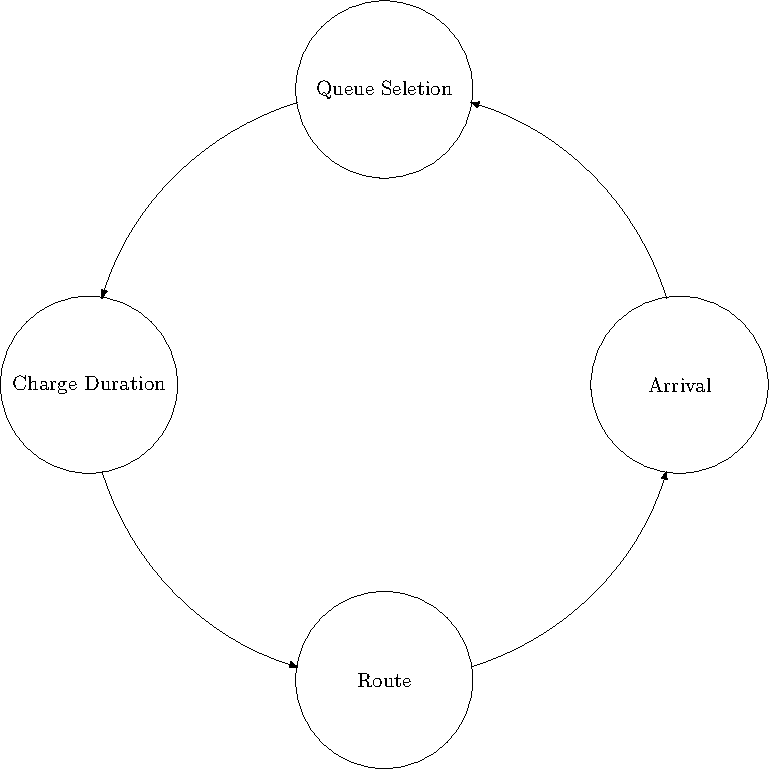
\includegraphics[width=0.7\textwidth]{./img/visit.pdf}
\end{center}
\end{frame}

\begin{frame}[label={sec:orgb90209d}]{Mixed Integer Linear Programming}
\begin{align*}
\text{max }        &J = \sum_j c_j x_j + \sum_k d_k y_k&         &               \\
\text{subject to } &\sum_j a_{ij} x_j + \sum_k g_{ik} y_k \le b_i&  &(i = 1,2,...,m)\\
                  &x_j \ge 0&                              &(j = 1,2,...,n)\\
                  &y_k \in \mathbb{Z^+}&                   &(k = 1,2,...,n)\\
\end{align*}

\begin{itemize}
\item \(J\): Objective function
\item \(x_j \in \mathbb{R}\) and \(y_k \in \mathbb{Z}^+\): Decision Variables
\item \(c_j, d_k, a_{ij}, g_{ik}, b_i \in \mathbb{R}\): Parameters
\end{itemize}
\end{frame}

\begin{frame}[label={sec:org98a805e}]{The Berth Allocation Problem\footnote{\url{https://www.mdpi.com/2077-1312/11/7/1280}}}
\begin{figure}[htpb]
\centering
    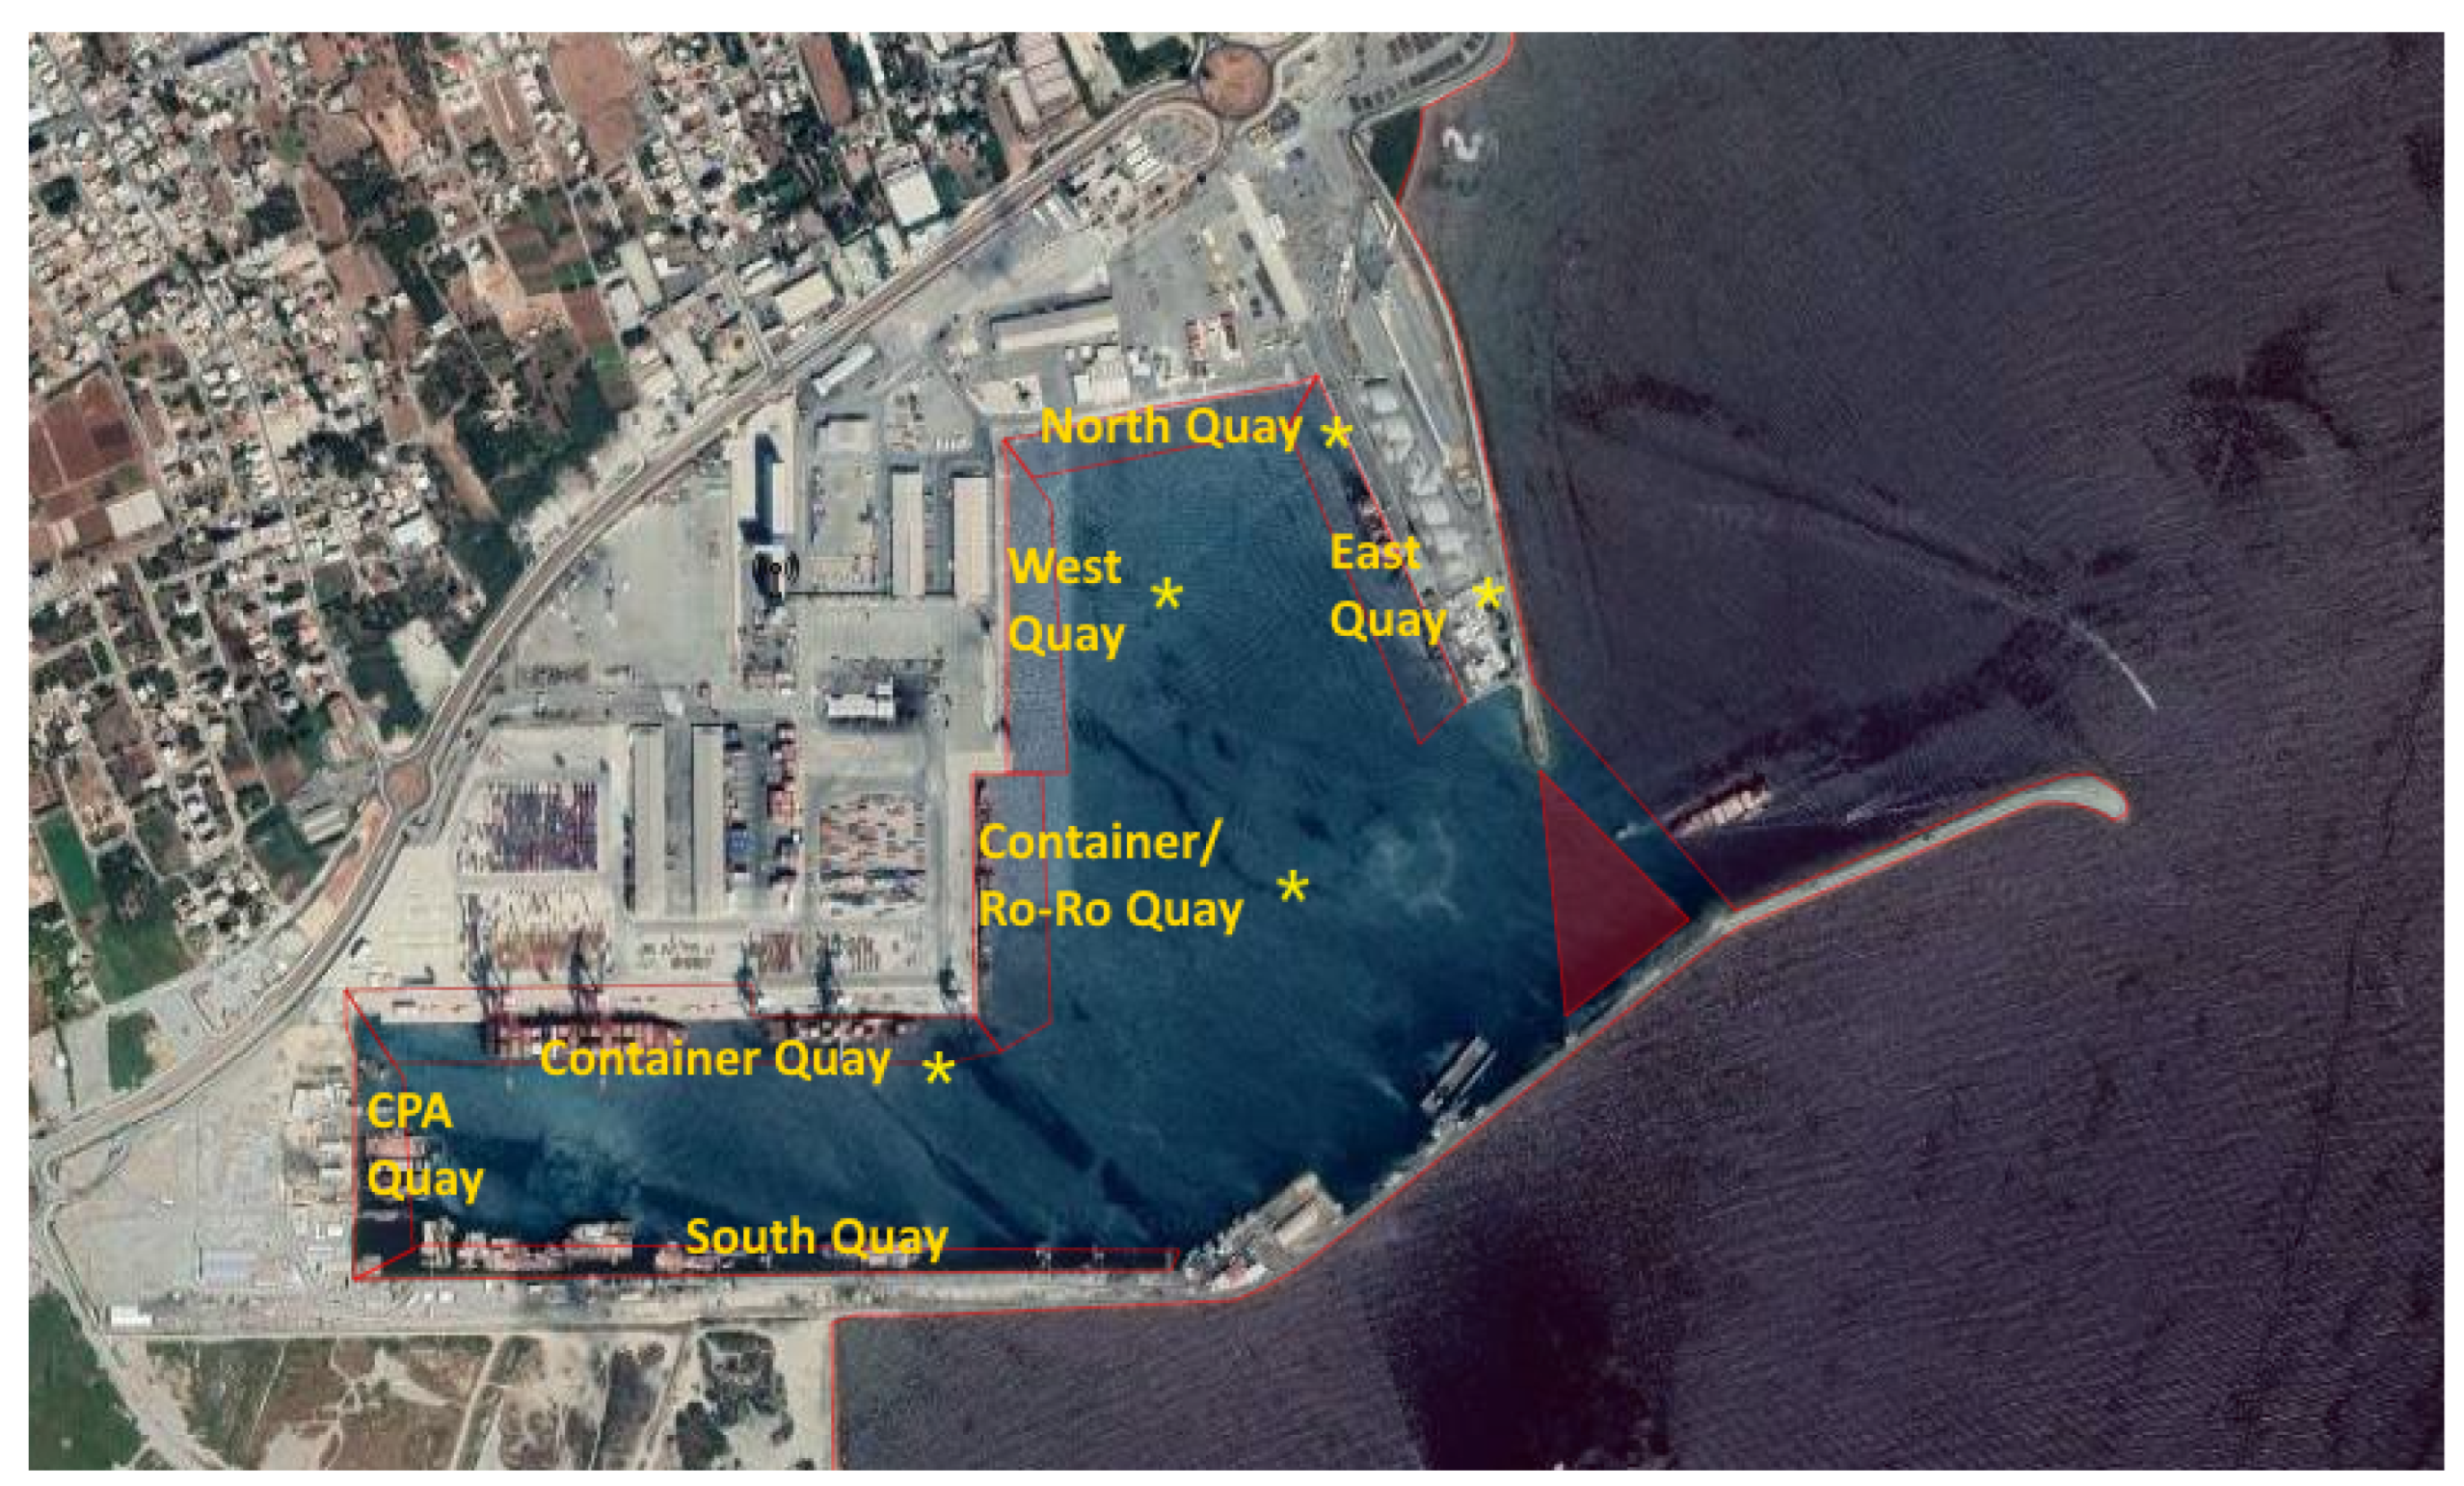
\includegraphics[width=0.9\textwidth]{img/berthing-sky-picture}
\end{figure}
\end{frame}

\begin{frame}[label={sec:org5060595}]{The Berth Allocation Problem}
\begin{columns}
\begin{column}{0.5\columnwidth}
\begin{itemize}
\item Vessels move down toward the quay
\item Recieve service
\item Exit to the right
\end{itemize}
\end{column}

\begin{column}{0.5\columnwidth}
\begin{figure}[htpb]
\centering
    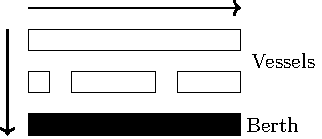
\includegraphics{img/bap}
    \label{subfig:bapexample}
\end{figure}
\end{column}
\end{columns}
\end{frame}

\begin{frame}[label={sec:org42a2cf6}]{The Berth Allocation Problem}
\begin{itemize}
\item A variant of the rectangle packing problem
\item Solves the problem of optimally assigning incoming vessels to be serviced
\begin{itemize}
\item \(\mathbb{O}\): Spatiotemporal allocations for vessels
\item \(O\): Time horizon and berthing space
\end{itemize}
\end{itemize}
\end{column}

\begin{column}{0.3\columnwidth}
\begin{figure}[htpb]
\centering
    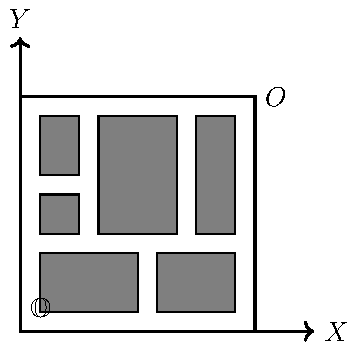
\includegraphics[width=\textwidth]{img/spatiotemporal-packing}
\end{figure}
\end{column}
\end{columns}
\end{frame}

\begin{frame}[label={sec:org211e9ec}]{The Position Allocation Problem}
\begin{columns}
\begin{column}{0.5\columnwidth}
\begin{itemize}
\item Service flow is left to right
\item Single charger type
\item All arrivals are considered unique
\item Service times are assumed to be known
\end{itemize}
\end{column}

\begin{column}{0.5\columnwidth}
\begin{figure}[htpb]
\centering
    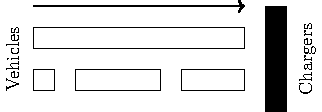
\includegraphics{img/pap}
    \label{subfig:papexample}
\end{figure}
\end{column}
\end{columns}
\end{frame}

\section{The Position Allocation Problem Approach With Linear Battery Dynamic}
\label{sec:org2414ef1}
\begin{frame}[label={sec:org146f773}]{Requirements For BEB Implementation}
\begin{itemize}
\item Charges must be able to be tracked
\item Service time is unknown
\item Accommodate chargers of different speeds
\item Minimize charger count
\item Minimize consumption cost
\item Encourage slow charger use for battery health
\end{itemize}
\end{frame}

\begin{frame}[label={sec:orgab8250e}]{Objective Function}
\begin{equation*}
\label{eq:objective}
	\min \sum_{i=1}^{n_V} \sum_{q=1}^{n_Q} \Big( w_{iq} m_q + g_{iq} \epsilon_q \Big)
\end{equation*}

\begin{itemize}
\item \(w_{iq} m_q\): Assignment cost
\item \(g_{iq} \epsilon_q\): Consumption cost
\end{itemize}
\end{frame}

\begin{frame}[label={sec:orgcca17be}]{Packing Constraints}
\begin{columns}
\begin{column}{0.5\columnwidth}
\begin{equation*}
    u_j - u_i - s_i - (\sigma_{ij} - 1)T \geq 0
\end{equation*}
\begin{equation*}
    v_j - v_i - (\psi_{ij} - 1)n_Q \geq 1
\end{equation*}
\begin{equation*}
    \sigma_{ij} + \sigma_{ji} \leq 1
\end{equation*}
\begin{equation*}
    \psi_{ij} + \psi_{ji} \leq 1
\end{equation*}
\begin{equation*}
    \sigma_{ij} + \sigma_{ji} + \psi_{ij} + \psi_{ji} \geq 1
\end{equation*}
\end{column}
\end{columns}
\end{frame}

\begin{frame}[label={sec:org53484e4}]{Packing Constraints}
\begin{columns}
\begin{column}{0.5\columnwidth}
\begin{itemize}
\item Used to ensure that individual rectangles do not overlap
\item \(\sigma_{ij}\) establishes temporal ordering when active
\item \(\psi_{ij}\) establishes spacial ordering when active
\end{itemize}
\end{column}

\begin{column}{0.5\columnwidth}
\begin{figure}
    \centering
    \scalebox{0.33}{
      \centering
        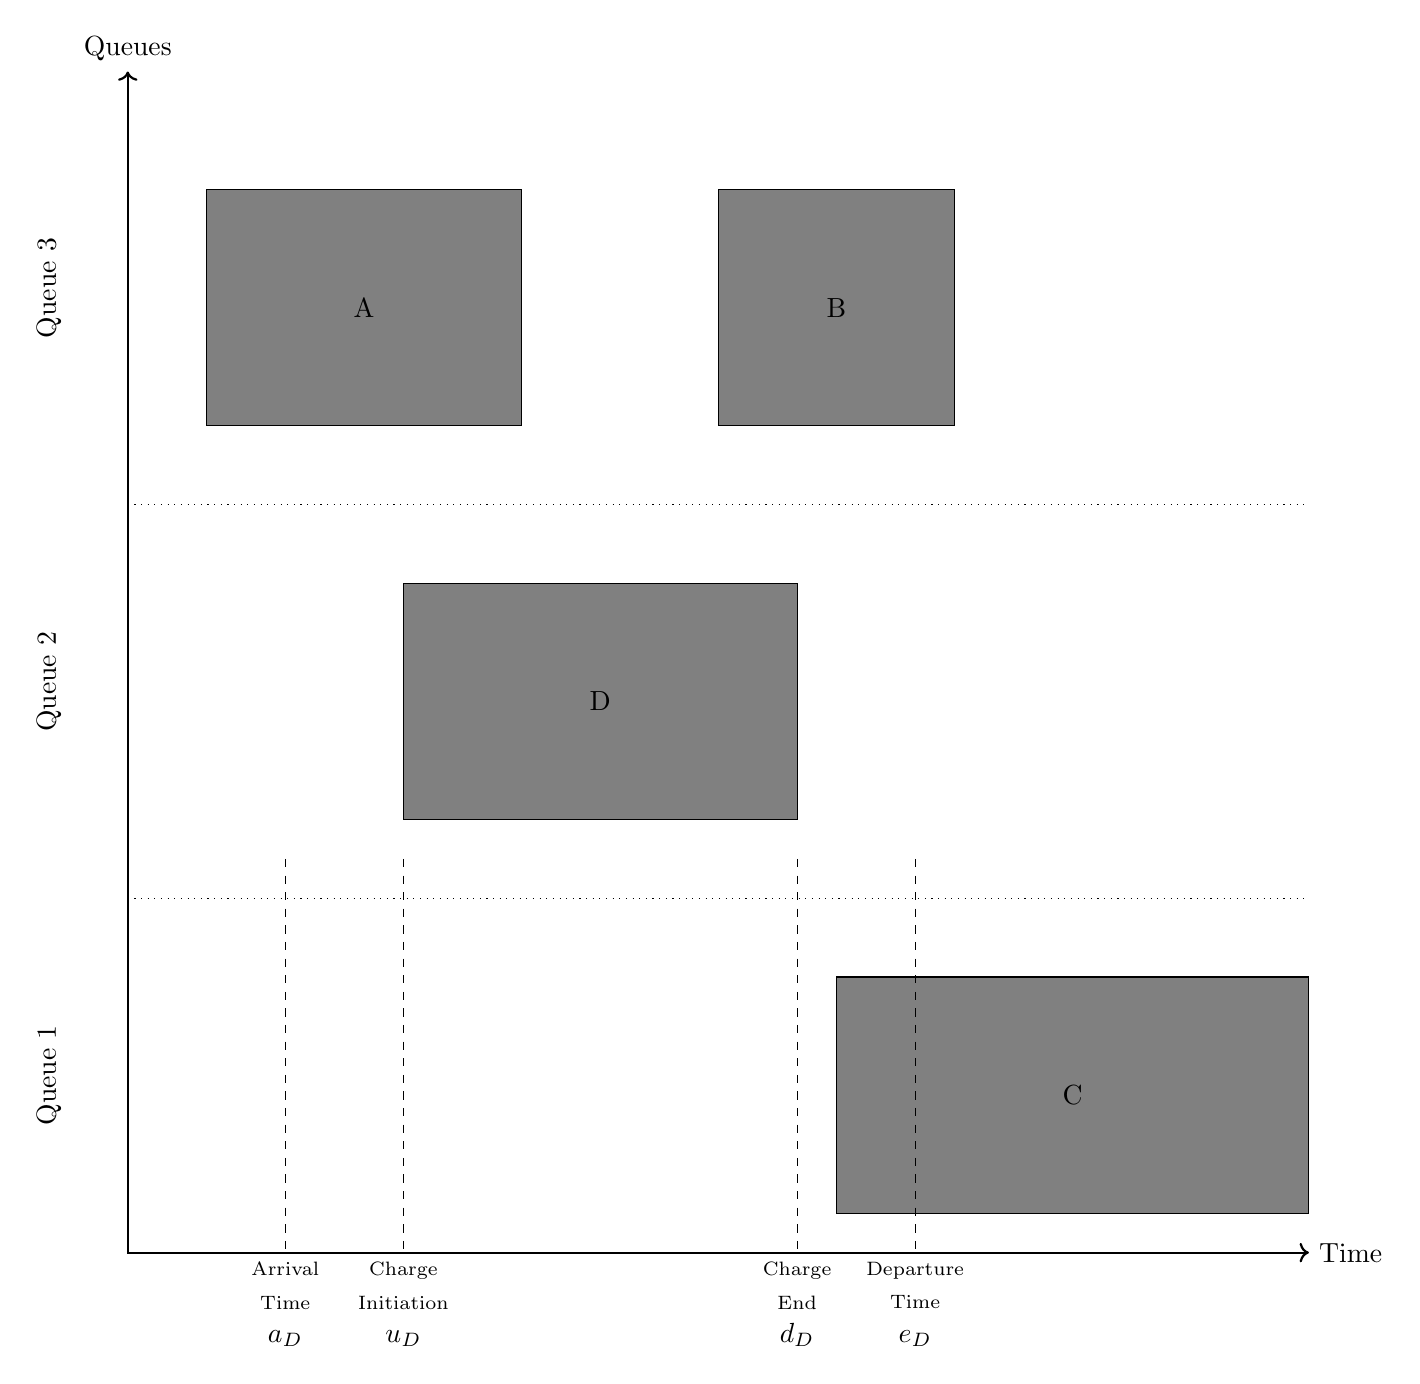
\begin{tikzpicture}
          % Variables
          \def \arrx   {2.0}
          \def \initx  {3.5}
          \def \endx   {8.5}
          \def \depx   {10.0}
          \def \yshift {5}

          % Axis
          \draw [thick,<->] (0,15) node[above]{Queues} -- (0,0) -- (15,0) node[right]{Time};

          % Rectangles
          \node[rectangle, draw, fill=gray, minimum width=4cm, minimum height = 3cm] at (3,12) {A};
          \node[rectangle, draw, fill=gray, minimum width=3cm, minimum height = 3cm] at (9,12) {B};
          \node[rectangle, draw, fill=gray, minimum width=5cm, minimum height = 3cm] at (6,7) {D};
          \node[rectangle, draw, fill=gray, minimum width=6cm, minimum height = 3cm] at (12,2) {C};

          % X-axis labels
          \node [below,align=center] at (\arrx,0) {\scriptsize Arrival     \\ \scriptsize Time \\ $a_D$};
          \node [below, align=center] at (\initx,0) {\scriptsize Charge    \\ \scriptsize Initiation  \\ $u_D$};
          \node [below, align=center] at (\endx,0) {\scriptsize Charge     \\ \scriptsize End \\ $d_D$};
          \node [below, align=center] at (\depx,0) {\scriptsize Departure  \\ \scriptsize Time \\ $e_D$};

          % Y-axis labels
          \node[rotate=90] at (-1, 2.25) {Queue 1};
          \node[rotate=90] at (-1, 7.25) {Queue 2};
          \node[rotate=90] at (-1, 12.25) {Queue 3};

          % Vertical lines
          \draw[dashed] (\arrx,\yshift)--(\arrx,0);
          \draw[dashed] (\initx,\yshift)--(\initx,0);
          \draw[dashed] (\endx,\yshift)--(\endx,0);
          \draw[dashed] (\depx,\yshift)--(\depx,0);

          % Horizontal lines
          \draw[dotted] (0, 4.5) -- (15, 4.5);
          \draw[dotted] (0, 9.5) -- (15, 9.5);

        \end{tikzpicture}
      }
      \label{fig:spacial-and-temporal-constr}
\end{figure}
\end{column}
\end{columns}
\end{frame}

\begin{frame}[label={sec:orgfeaf21c}]{Packing Constraints}
\begin{columns}
\begin{column}{0.5\columnwidth}
\begin{itemize}
\item Calculates the charge duration
\item Ensures the arrival time is before the initial charge time
\item The initial charge time must be early enough as to not go over the time horizon
\item The detach time must be before the departure time
\end{itemize}
\end{column}

\begin{column}{0.5\columnwidth}
\begin{equation*}
    s_i + u_i = d_i
\end{equation*}
\begin{equation*}
    a_i \leq u_i \leq (T - s_i)
\end{equation*}
\begin{equation*}
    d_i \leq \tau_i
\end{equation*}
\end{column}
\end{columns}
\end{frame}

\begin{frame}[label={sec:orge57c021}]{Linear Battery Dynamic Constraints}
\begin{columns}
\begin{column}{0.5\columnwidth}
\begin{itemize}
\item Calculates the charge for the next visit
\item Ensures the current charge is above the minimum charge threshold
\item Ensures the current charge is below the battery capacity
\end{itemize}
\end{column}

\begin{column}{0.5\columnwidth}
\begin{equation*}
    \eta_i + \sum_{q=1}^{n_Q} g_{iq} r_q - \Delta_i = \eta_{\gamma_i}
\end{equation*}
\begin{equation*}
    \eta_i + \sum_{q=1}^{n_Q} g_{iq} r_q - \Delta_i \geq \nu_{\Gamma_i} \kappa_{\Gamma_i}
\end{equation*}
\begin{equation*}
    \eta_i + \sum_{q=1}^{n_Q} g_{iq} r_q \leq \kappa_{\Gamma_i}
\end{equation*}
\end{column}
\end{columns}
\end{frame}

\begin{frame}[label={sec:orgfe1de62}]{Bilinear Linearization Constraints}
\begin{columns}
\begin{column}{0.5\columnwidth}
\begin{itemize}
\item Linearization of bilinear terms
\end{itemize}

\begin{equation*}
    \label{eq:giq_cases}
    g_{iq} =
    \begin{cases}
        s_i & w_{iq} = 1 \\
        0 & w_{iq} = 0
    \end{cases}.
\end{equation*}
\end{column}


\begin{column}{0.5\columnwidth}
\begin{equation*}
    s_i - (1 - w_{iq})M \leq g_{iq}
\end{equation*}
\begin{equation*}
    s_i \geq g_{iq}
\end{equation*}
\begin{equation*}
    Mw_{iq} \geq g_{iq}
\end{equation*}
\begin{equation*}
    0 \leq g_{iq}
\end{equation*}
\end{column}
\end{columns}
\end{frame}

\begin{frame}[label={sec:org8a5abcf}]{Charging Queue Constraints}
\begin{columns}
\begin{column}{0.5\columnwidth}
\begin{itemize}
\item Ensure only one queue is selected per visit
\item Convert vector representation of queue selection to an integer
\end{itemize}
\end{column}

\begin{column}{0.5\columnwidth}
\begin{equation*}
    \sum_{q=1}^{n_Q} w_{iq} = 1
\end{equation*}
\begin{equation*}
    v_i = \sum_{q=1}^{n_Q} qw_{iq}
\end{equation*}
\end{column}
\end{columns}
\end{frame}


\begin{frame}[label={sec:org7368a60}]{Results}
\begin{itemize}
\item Executed for 7200 seconds (2 hours)
\item \(T = 24\)
\item \(n_V = 338\)
\item \(n_A = 35\)
\item \(\alpha_i = 90\%\);  \(\nu_i = 20\%\);  \(\beta_i = 70\%\)
\item \(\forall q \in \{n_B + 1, n_B + 2,..., n_B + n_C \}; m_q = 1000q\)
\end{itemize}
\end{frame}

\begin{frame}[label={sec:orge0b2434}]{Results}
\begin{figure}[htpb]
\centering
    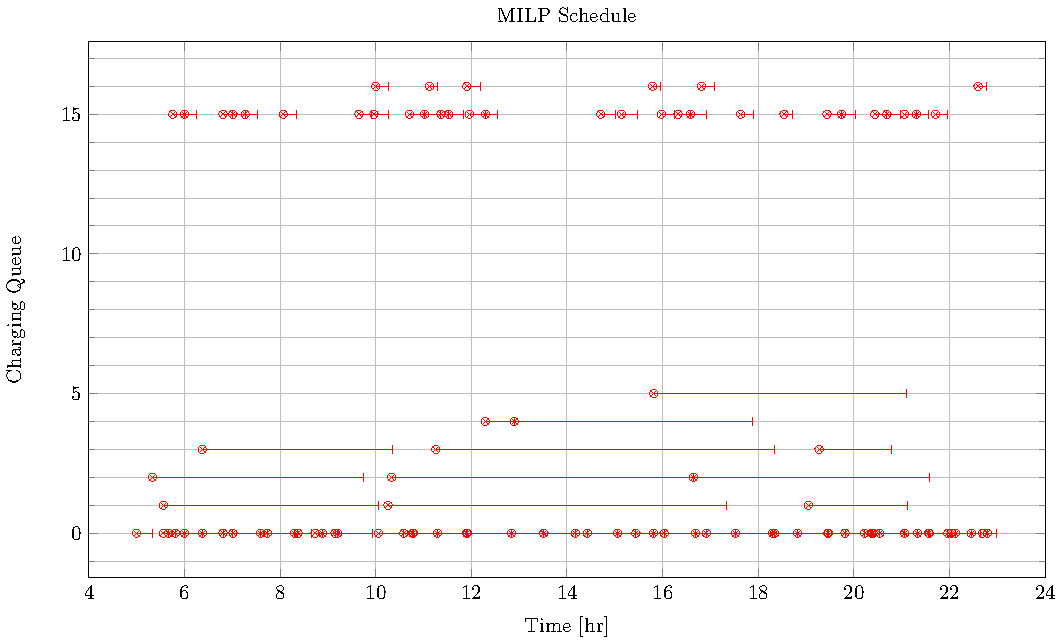
\includegraphics[width=\textwidth]{img/schedule-milp-pap}
\end{figure}
\end{column}

\begin{column}{0.5\columnwidth}
\begin{figure}[htpb]
\centering
    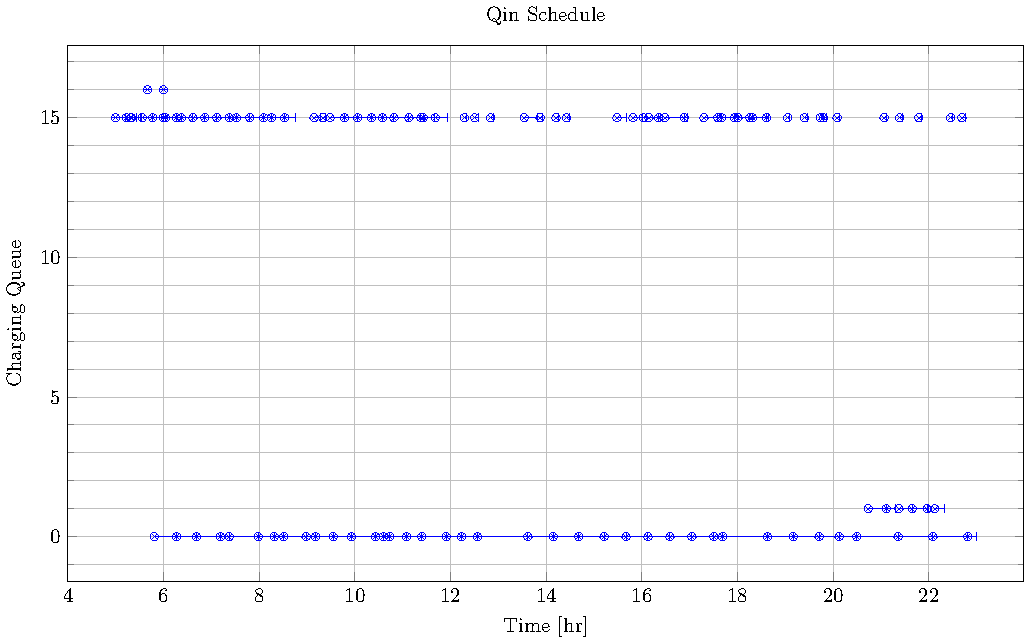
\includegraphics[width=\textwidth]{img/schedule-qin}
\end{figure}
\end{column}
\end{columns}
\end{frame}

\begin{frame}[label={sec:org4ee59dd}]{Results}
\begin{figure}[htpb]
\centering
    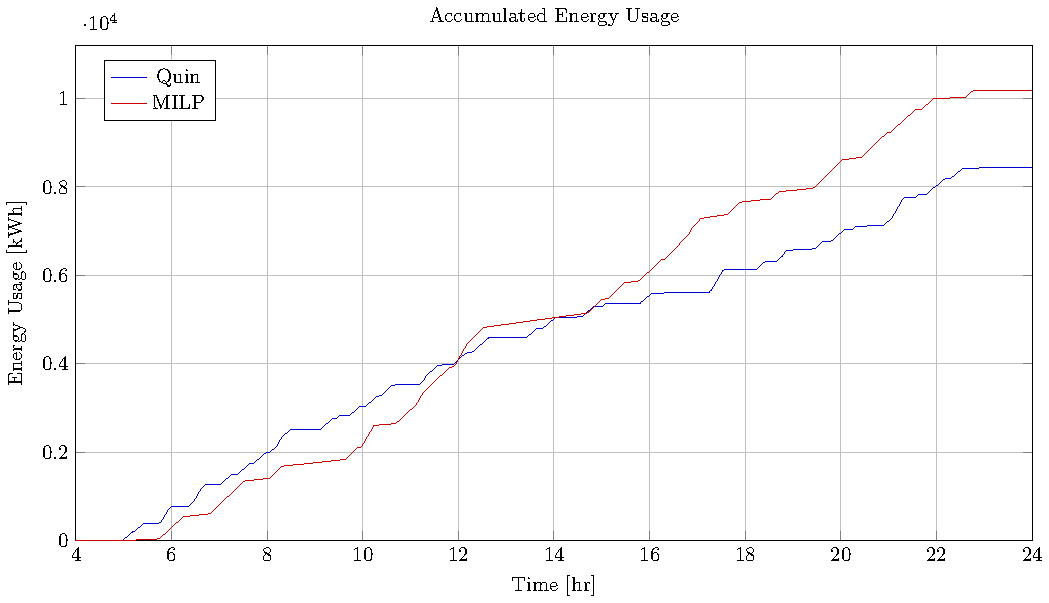
\includegraphics[width=\textwidth]{img/energy-milp-pap}
\end{figure}
\end{column}

\begin{frame}[label={sec:org45e043c}]{Results}
\begin{figure}[htpb]
\centering
    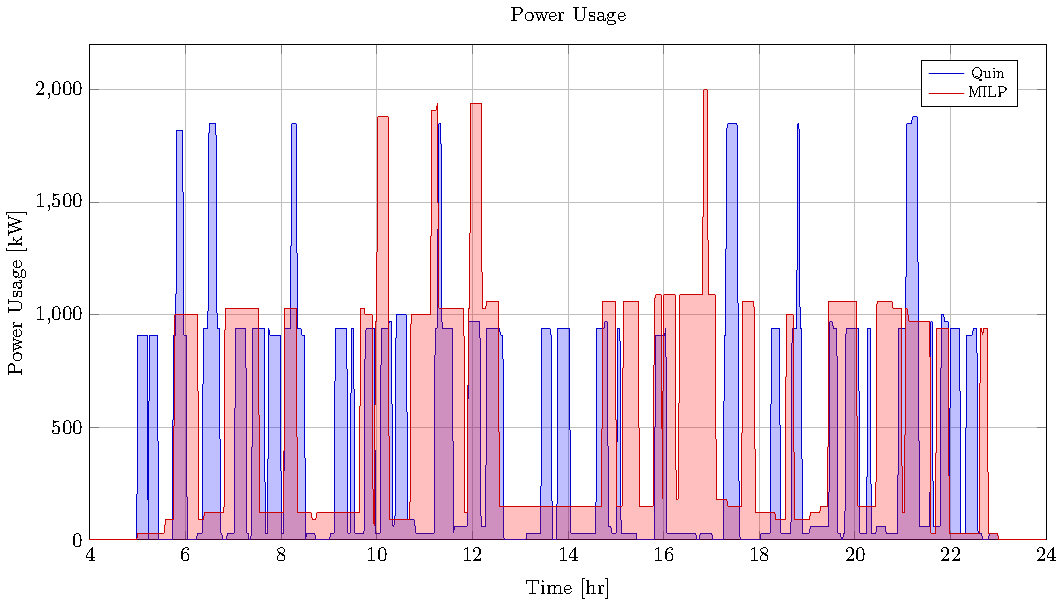
\includegraphics[width=\textwidth]{img/power-milp-pap}
\end{figure}
\end{column}
\end{columns}
\end{frame}

\section{The Simulated Annealing Approach With Linear Battery Dynamics}
\label{sec:org9b6f730}
\begin{frame}[label={sec:org7c50f9d}]{Simulated Annealing}
\begin{itemize}
\item Named after its analogized process where a crystalline solid is heated then allowed to cool at a slow rate until it achieves its most regular possible crystal lattice configuration
\item The algorithm is often applied to problems that contain many local solutions as it employs a stochastic approach that explores the solution space for an approximate global optimum.
\item Within the SA process there are three key components
\begin{itemize}
\item Cooling Schedule
\item Acceptance Criteria
\item Generation Mechanisms
\end{itemize}
\end{itemize}
\end{frame}
\begin{frame}[label={sec:org3b3b6e3}]{Cooling Schedule}
\begin{columns}
\begin{column}{0.5\columnwidth}
\begin{itemize}
\item The cooling equation models the rate at which the temperature decreases over time in the SA process.
\item The temperature is high, SA encourages exploration. As the temperature decreases, exploitation is encouraged.
\end{itemize}
\end{column}

\begin{column}{0.5\columnwidth}
\begin{figure}[t!]
  \centering 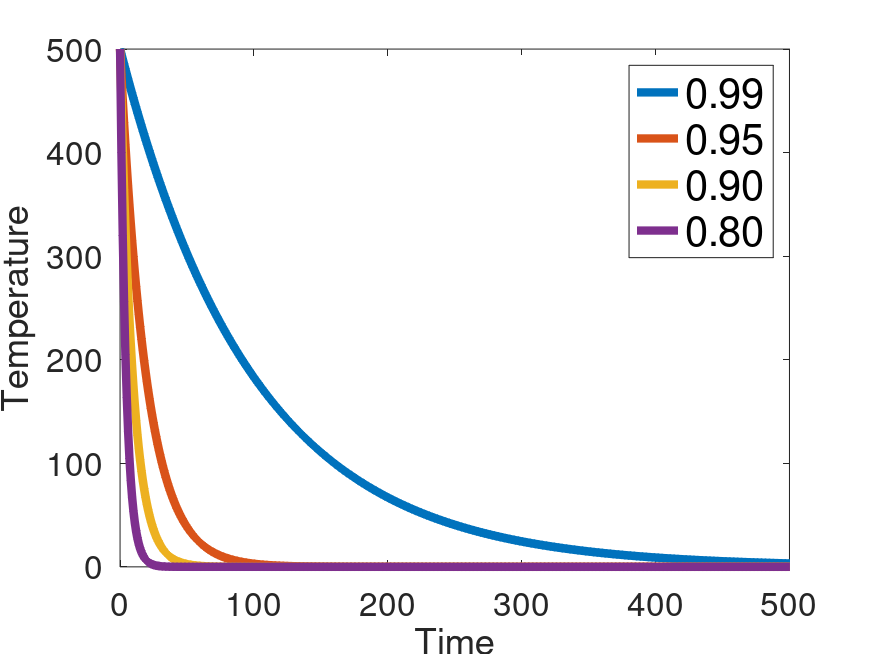
\includegraphics[width=0.9\textwidth]{img/geometric.png}
  \label{fig:geometric}
\end{figure}

\begin{equation*}
t_m = \beta t_{m-1}
\end{equation*}
\end{column}
\end{columns}
\end{frame}

\begin{frame}[label={sec:org81a1b10}]{Acceptance Criteria}
\begin{equation}
\label{eq:candaccept}
f(\mathbb{I},\bar{\mathbb{I}},t_m) =
\begin{cases}
  1                   & \Delta E > 0 \\
  e^{- \frac{\Delta E}{t_m}} & \text{otherwise}
\end{cases}
\end{equation}
\end{frame}

\begin{frame}[label={sec:orgc6dca5f}]{Generation Mechanisms - Primitive Functions}
\begin{itemize}
\item New Visit: Move a bus from a wait queue to charge queue
\item Slide Visit: Change the charge duration of a visit
\item New Charger: Move a visit to a new charger
\item Wait: Move a visit to its idle queue
\item New Window: Execute Wait then New Visit primitives
\end{itemize}
\end{frame}

\begin{frame}[label={sec:org852e0ed}]{New Visit}
\begin{algorithm}[H]
  \scriptsize
  \caption{New visit algorithm}
  \label{alg:new-visit}
  \LinesNumbered
  \TitleOfAlgo{New Visit}
  \KwIn{$\Sol$}
  \KwOut{$\bar{\Sol}$}

  \SetKwFunction{Union}{Union}
  \SetKwFunction{findFreeTime}{findFreeTime}

  \Begin
    {
      $i \leftarrow \Sol_{i}$\tcc*{Extract visit index}
      $a \leftarrow \I_{i.a}$\tcc*{Extract the arrivial time for visit $i$}
      $e \leftarrow \I_{i.e}$\tcc*{Extract the departure time for visit $i$}
      $q \leftarrow \I_{i.q}$\tcc*{Extract the current charge queue for visit $i$}
      $\bar{q} \leftarrow \mathcal{U}_{Q}$\tcc*{Select a random charging queue with a uniform distribution}
      $C \leftarrow \mathcal{U}_{\C_q}$\tcc*{Select a random time slice from $\C_q$}

      \If(\tcc*[f]{If there is time available in $C_q^j$}){($\bar{C}, \bar{u}, \bar{d}$) $\leftarrow$ \findFreeTime{$C, i, q, a, e$} $\not\in \varnothing$}
         {
           \Return{($i, (\bar{q},\bar{u},\bar{d}),\bar{C}$)}\tcc*[f]{Return visit}
         }

         \Return{($\varnothing$)}\tcc*{Return nothing}
    }
\end{algorithm}
\end{frame}

\begin{frame}[label={sec:org9e6d910}]{Slide Visit}
\begin{algorithm}[H]
  \scriptsize
  \caption{Slide Visit Algorithm} \label{alg:slide-visit}
  \LinesNumbered
  \TitleOfAlgo{Slide Visit}
  \KwIn{$\Sol$}
  \KwOut{$\bar{\Sol}$}

    \SetKwFunction{Purge}{Purge}

    \Begin
    {
      $(i, \I, \bar{\C}) \leftarrow$\Purge{$\Sol$}\tcc*{Purge visit $i$ from charger availibility matrix}
      $C \leftarrow \bar{C}_{i.q_i}$\tcc*{Get the time availability of the purged visit}

      \tcc{If there is time available in $C$}
      \If{($\bar{C}, \bar{u}, \bar{d}$) $\leftarrow$ \findFreeTime{$C$, $\Sol_i$, $\I_q$, $\I_{i.a}, \I_{i.e}$} $\not\in \varnothing$}
      {
        \Return{($i, \I, (\I_{i.q_i},\bar{u},\bar{d}),\bar{C}$)}\tcc*[f]{Return updated visit}
      }

        \Return{($\varnothing$)}\tcc*{Return nothing}
    }
  \end{algorithm}
\end{frame}

\begin{frame}[label={sec:org796a8d2}]{New Charger}
\begin{algorithm}[H]
  \scriptsize
  \caption{New Charger Algorithm} \label{alg:new-charger} \LinesNumbered \TitleOfAlgo{New Charger} \KwIn{$\Sol$}
  \KwOut{$\bar{\Sol}$}

    \SetKwFunction{Purge}{Purge}

    \Begin
    {
      $(i, \I, \bar{\C}) \leftarrow$\Purge{$\Sol$}\tcc*{Purge visit $i$ from charger availibility matrix}
      $q \leftarrow \mathcal{U}_{Q}$\tcc*{Select a random charging queue with a uniform distribution}

      \If(\tcc*[f]{If there is time available in $C_{q}$}){($\bar{C}, \bar{u}, \bar{d}$) $\leftarrow$ \findFreeTime{$\bar{\C}_{i.q}$, $\Sol_i$, $\I_q$, $\I_{i.a}, \I_{i.e}$} $\not\in \varnothing$}
      {
        \tcc{Return visit, note $u$ and $d$ are the original inital/final charge times.}
        \Return{($i, \I, (q,\I_{i.u}, \I_{i.d}),\bar{\C}$)}
      }

      \Return{($\varnothing$)}\tcc*{Return nothing}
    }
  \end{algorithm}
\end{frame}

\begin{frame}[label={sec:org011586c}]{Wait}
\begin{algorithm}[H]
\scriptsize
\caption{Wait algorithm} \label{alg:wait}
    \LinesNumbered
    \TitleOfAlgo{Wait}
    \KwIn{$\Sol$}
    \KwOut{$\bar{\Sol}$}

    \SetKwFunction{Purge}{Purge}

    \Begin
    {
      $(i, \I, \bar{\C}) \leftarrow$\Purge{$\Sol$}\tcc*{Purge visit $i$ from charger availibility matrix}
      $\bar{\C}'_{\I_{i.\Gamma_i}} \leftarrow \C' \cup \{[\I_{i.a}, \I_{i.e}]\}$\tcc*{Update the charger availability matrix for wait queue $\bar{\C}_{i.q_i}$}
      \Return{$(i, \I, (\I_{i.b}, \I_{i.a}, \I_{i.e}), \bar{\C})$}\tcc*[f]{Return visit}
    }
  \end{algorithm}
\end{frame}

\begin{frame}[label={sec:org2906760}]{New Window}
\begin{algorithm}[H]
  \scriptsize
  \caption{New window algorithm} \label{alg:new-window}
  \LinesNumbered
  \TitleOfAlgo{New Window}
  \KwIn{$\Sol$}
  \KwOut{$\bar{\Sol}$}

  \SetKwFunction{NewVisit}{NewVisit}
  \SetKwFunction{Wait}{Wait}

  \Begin
  {
    $\bar{\Sol} \leftarrow$\Wait{$\Sol$}\tcc*{Assign visit to its respective idle queue}
    \If(\tcc*[f]{Add visit $i$ back in randomly})
       {
         $\bar{\bar{\Sol}} \leftarrow$ \NewVisit{$\bar{\Sol}$} $\not\in \varnothing$
       }
       {
         \Return{$\bar{\bar{\Sol}}$} \tcc*[f]{Return visit}
       }

       \Return{($\varnothing$)}\tcc*{Return nothing}
  }
\end{algorithm}
\end{frame}

\begin{frame}[label={sec:org189b6d6}]{Generation Mechanisms - Wrapper Functions}
\begin{itemize}
\item Charge Schedule Generation: Iterate through each visit and execute New Visit
\item Perturb Schedule: Randomly execute one of the primitives with a weighted distribution
\end{itemize}
\end{frame}

\begin{frame}[label={sec:org7169a88}]{Charge Schedule Generation}
\begin{algorithm}[H]
\scriptsize
\caption{Charge schedule generation algorithm} \label{alg:charge-schedule-generation}
    \LinesNumbered
    \TitleOfAlgo{Candidate Solution Generator}
    \KwIn{$\Sol$}
    \KwOut{$\bar{\Sol}$}

    \SetKwFunction{NewVisit}{NewVisit}

    \Begin
    {
        \tcc{Select an unscheduled BEB visit from a randomly indexed set of visits}
        \ForEach {$\I_i \in \I$}
        {
            ($i, \bar{\I}$, $\bar{\C}$) $\leftarrow$ \NewVisit{($\I_i$, $\I$, $\C$)}\tcc*{Assign the bus to a charger}
        }
            \Return{($0, \bar{\I}$, $\bar{\C}$)}
    }
  \end{algorithm}
\end{frame}

\begin{frame}[label={sec:org7efc9d5}]{Perturb Schedule}
\begin{center}
\scalebox{0.65}{
\begin{minipage}{1.5\linewidth}
\begin{algorithm}[H]
\scriptsize
\caption{Perturb schedule algorithm} \label{alg:perturb-schedule}

    \LinesNumbered
    \TitleOfAlgo{Perturb Schedule}
    \KwIn{$\Sol$}
    \KwOut{$\bar{\Sol}$}

    \SetKwFunction{PGF}{PGF}

    \Begin
    {
        $p \leftarrow [false; n_A]$\tcc*{Create vector to track priority routes}
        $y^i \leftarrow [1.0; n_V]$\tcc*{Create weight vector for index selection}
        \tcc{Loop through the visits in reverse order}
        \ForEach{$\I_i \leftarrow \I_{|\I|} \text{ TO } \I_{1}$}
        {
            \tcc{If the current visit is part of a priority route}
            \If{$p_{\I_{i.b}} = true$}{$y^i_{\I_i} = y^i_{\I_{i.\xi}}$\;}
            \tcc{Else if the current visit's SOC does below the allowed threshold}
            \ElseIf{$\I_{i.\eta} \le \nu_{\I_{i.b}} \kappa_{\I_{i.b}}$}{
                $p_{\I_{i.b}} = true$\tcc*{Indicate the current BEB's routes are to be prioritized}
                $y^i_{\I_i} = \kappa_{\I_{i.b}} (\nu_{\I_{i.b}}\kappa_{\I_{i.b}} - \I_{i.\eta})$\tcc*{Calculate the weight of the current visit}
            }
        }
        $\I_i\leftarrow\; \W^{y^i}_{\I}$\tcc*{Select an index with a weighted distribution}
        $i \leftarrow\; \I_i$\tcc*{Extract visit index}
        $y^p \leftarrow [y^p_1, y^p_2, ...]$\tcc*{Define the weight of each primitive generator}
        $PGF \leftarrow\; \W^{y^p}_{[1,n_G]}$\tcc*{Select a generator function with weighted distribution}
        $\bar{\Sol} \leftarrow$ \PGF{($i$, $\I$, $\C$)}\tcc*{Excecute the generator function}
        \Return{($0, \bar{\I}$, $\bar{\C}$)}
    }
\end{algorithm}
\end{minipage}}
\end{center}
\end{frame}

\begin{frame}[label={sec:orged78099}]{Objective Function}
\begin{equation*}
  J(\mathbb{I}) = z_d p_d + \sum_{i=1}^{n_V} \Big[ \epsilon_{q_i}r_{q_i} + z_p \phi_i(\eta_i - \nu_{b_i} \kappa_{b_i}) + z_c r_{q_i} s_i \Big]
\end{equation*}

\begin{columns}
\begin{column}{0.5\columnwidth}
\begin{itemize}
\item Demand cost
\begin{itemize}
\item \(p_{T_p}[h] = \frac{1}{T_p} \sum_{h-\frac{T_p}{dt}+1}^h p_h\)
\item \(p_d = \max(p_{fix}, p_{max})\)
\item \(p_{max} = \max\limits_{h \in H}p_{T_p}[h]\)
\end{itemize}
\end{itemize}
\end{column}

\begin{column}{0.5\columnwidth}
\begin{itemize}
\item \(\epsilon_{q_i}r_{q_i}\): Assignment Cost
\item \(z_p \phi_i(\eta_i - \nu_{b_i} \kappa_{b_i})\): Penalty Function
\item \(z_c r_{q_i} s_i\): Consumption Cost
\end{itemize}
\end{column}
\end{columns}
\end{frame}

\begin{frame}[label={sec:org88b4215}]{Constraints}
\begin{columns}
\begin{column}{0.5\columnwidth}
\begin{equation*}
    \label{seq:c0}
    u_j - d_i - (\sigma_{ij} - 1)T \ge 0
\end{equation*}
\begin{equation*}
    \label{seq:c1}
    q_j - q_i - 1 - (\psi_{ij} - 1)Q \ge 0
\end{equation*}
\begin{equation*}
    \label{seq:c2}
    \sigma_{ij} + \sigma_{ji} \le 1
\end{equation*}
\begin{equation*}
   \label{seq:c3}
    \psi_{ij} + \psi_{ji} \le 1
\end{equation*}
\end{column}

\begin{column}{0.5\columnwidth}
\begin{equation*}
    \label{seq:c4}
    \sigma_{ij} + \sigma_{ji} + \psi_{ij} + \psi_{ji} \ge 1
\end{equation*}
\begin{equation*}
    \label{seq:c5}
    s_i = d_i - u_i
\end{equation*}
\begin{equation*}
    \label{seq:c6}
     \eta_{\xi_i} = \eta_{i} + r_{q_i}s_i - \Delta_i
\end{equation*}
\begin{equation*}
    \label{seq:c7}
    \kappa_{\Xi_i} \geq \eta_{i} + r_{q_i}s_i
\end{equation*}
\begin{equation*}
    \label{seq:c8}
    a_i \leq u_i \leq d_i \le e_i \le \mathcal{T}
\end{equation*}
\end{column}
\end{columns}
\end{frame}

\begin{frame}[label={sec:org0b8fbd7}]{Results - What Is In The Thesis}
\begin{center}
\begin{tabular}{lrr}
\alert{Model} & \alert{Execution Time} [s] & \alert{Iteration} [s]\\[0pt]
\hline
MILP & 3600 & N/A\\[0pt]
Quick & 2275.25 & 0.25\\[0pt]
Heuristic & 3640.4 & 0.4\\[0pt]
\end{tabular}
\end{center}

\begin{columns}
\begin{column}{0.5\columnwidth}
\begin{itemize}
\item \(T_0 = 99999\)
\item \(\beta = 0.999\)
\end{itemize}
\end{column}
\begin{column}{0.5\columnwidth}
\begin{itemize}
\item \(|t| = 3797\)
\item \(n_K = 500\)
\end{itemize}
\end{column}
\end{columns}
\end{frame}

\begin{frame}[label={sec:org636a468}]{Schedule- What Is In The Thesis}
\begin{figure}[htpb]
\centering
    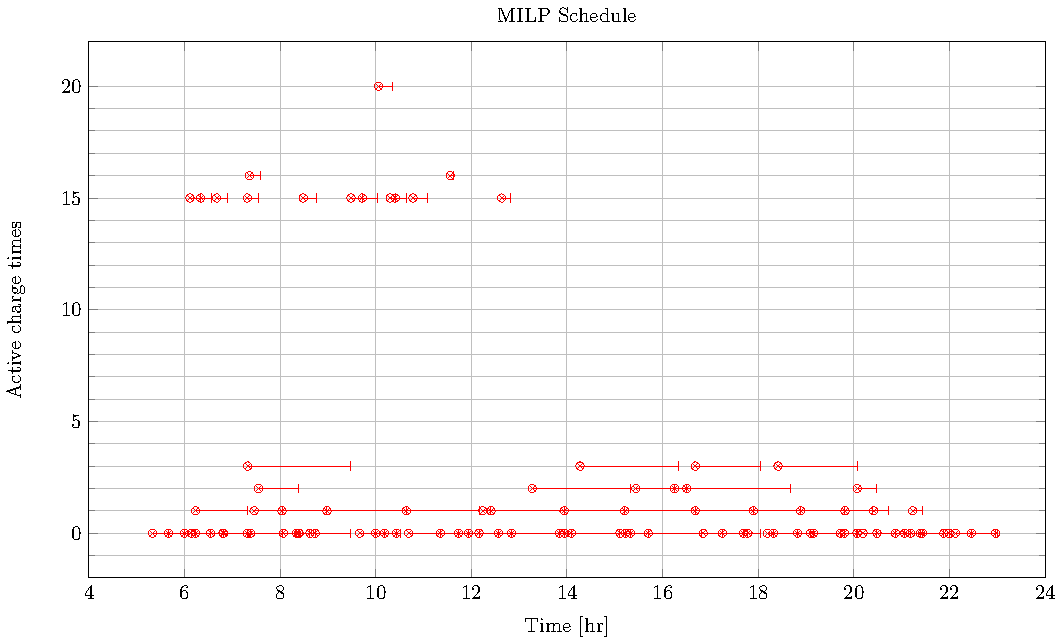
\includegraphics[width=0.6\textwidth]{img/sa-pap-paper-bad/schedule-milp}
\end{figure}
\begin{figure}[htpb]
\centering
    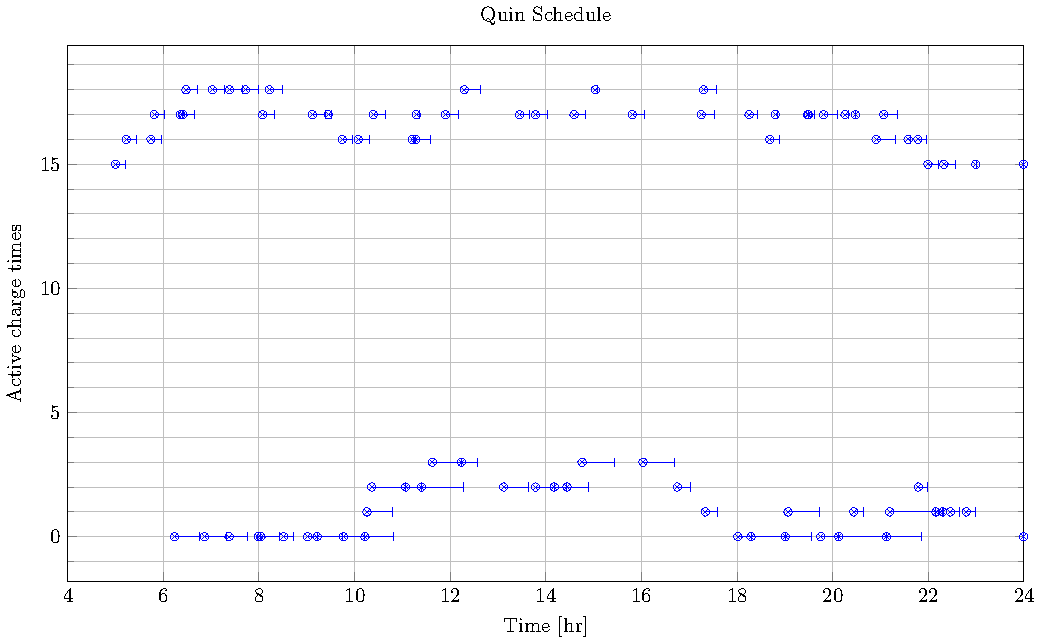
\includegraphics[width=0.6\textwidth]{img/sa-pap-paper-bad/schedule-quinn}
\end{figure}
\end{frame}

\begin{frame}[label={sec:org77bf612}]{Schedule - What Is In The Thesis}
\begin{figure}[htpb]
\centering
    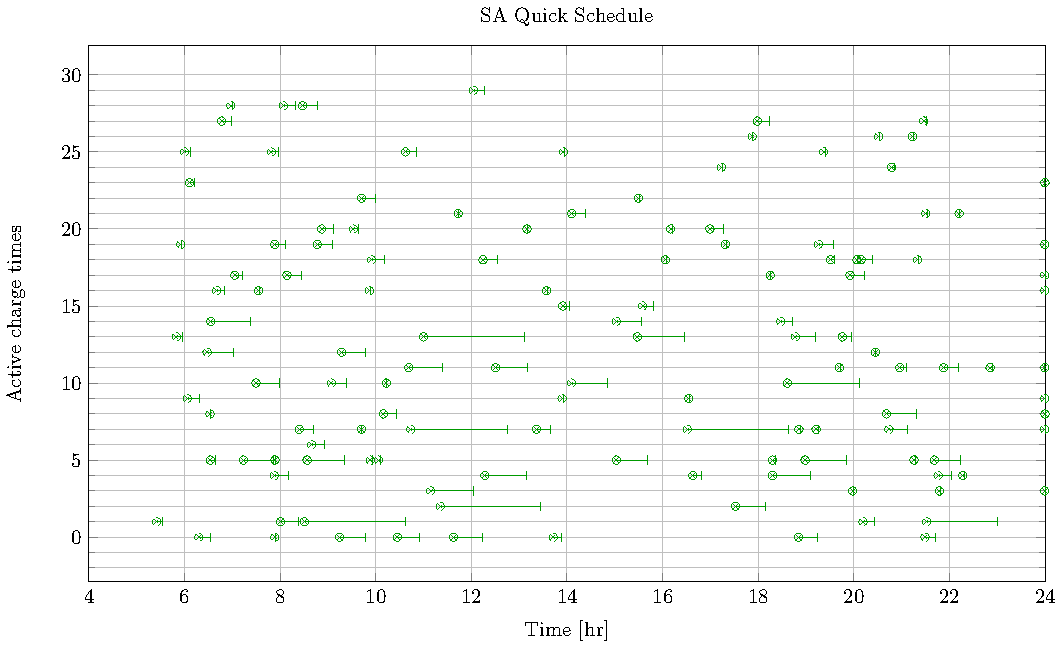
\includegraphics[width=0.6\textwidth]{img/sa-pap-paper-bad/schedule-sa-quick}
\end{figure}
\begin{figure}[htpb]
\centering
    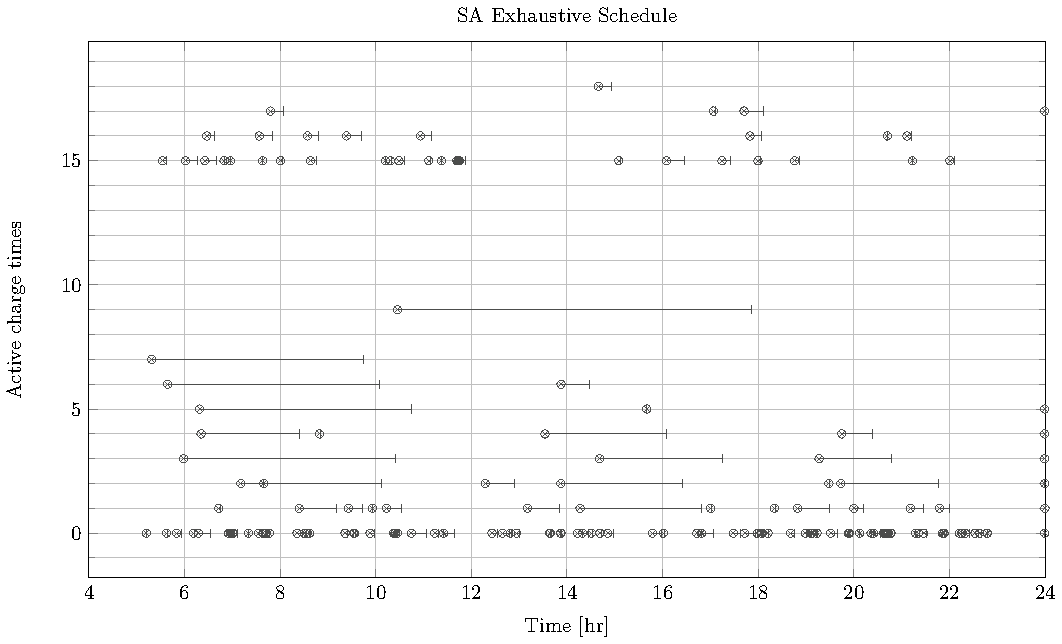
\includegraphics[width=0.6\textwidth]{img/sa-pap-paper-bad/schedule-sa-heuristic}
\end{figure}
\end{frame}

\begin{frame}[label={sec:org24491af}]{Charger Count - What Is In The Thesis}
\begin{figure}[htpb]
\centering
    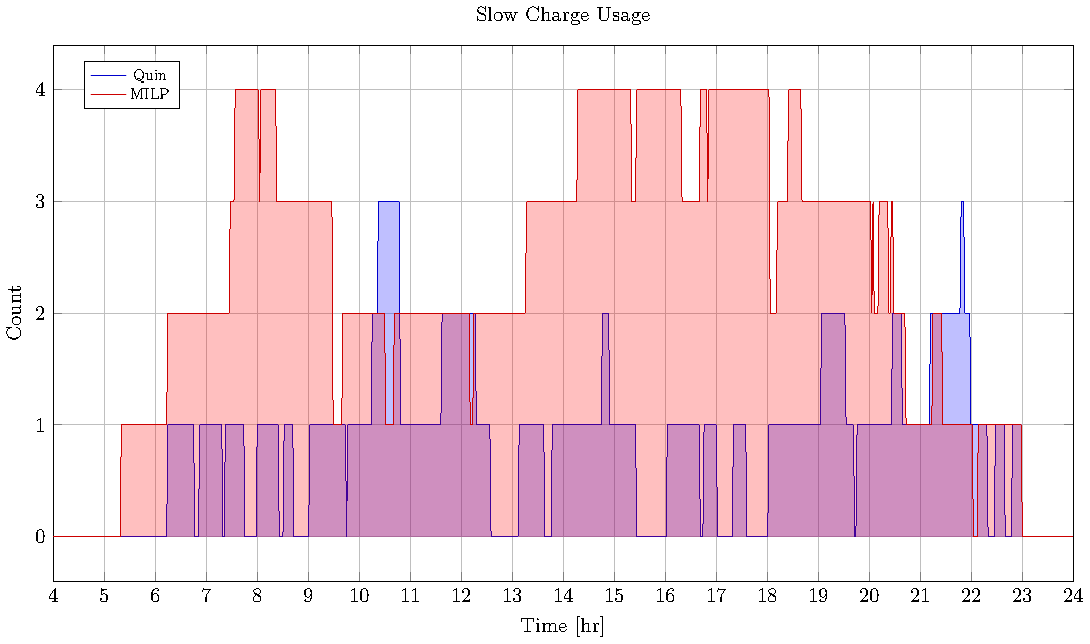
\includegraphics[width=0.6\textwidth]{img/sa-pap-paper-bad/charger-count-slow-milp-qin}
\end{figure}
\begin{figure}[htpb]
\centering
    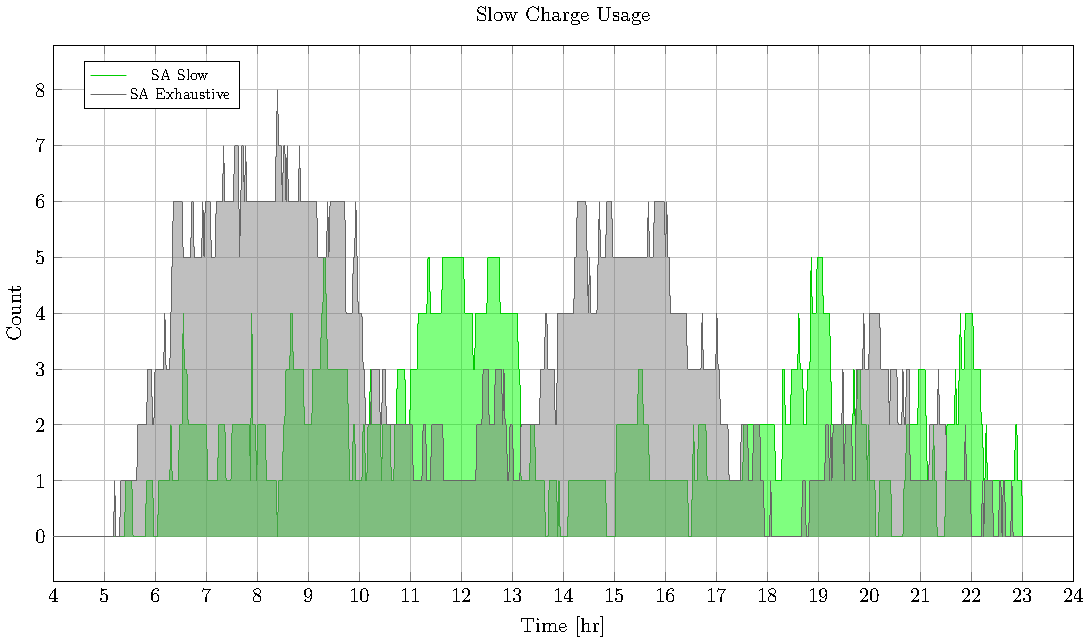
\includegraphics[width=0.6\textwidth]{img/sa-pap-paper-bad/charger-count-slow-sa}
\end{figure}
\end{frame}

\begin{frame}[label={sec:orgcd6db83}]{Charger Count - What Is In The Thesis}
\begin{figure}[htpb]
\centering
    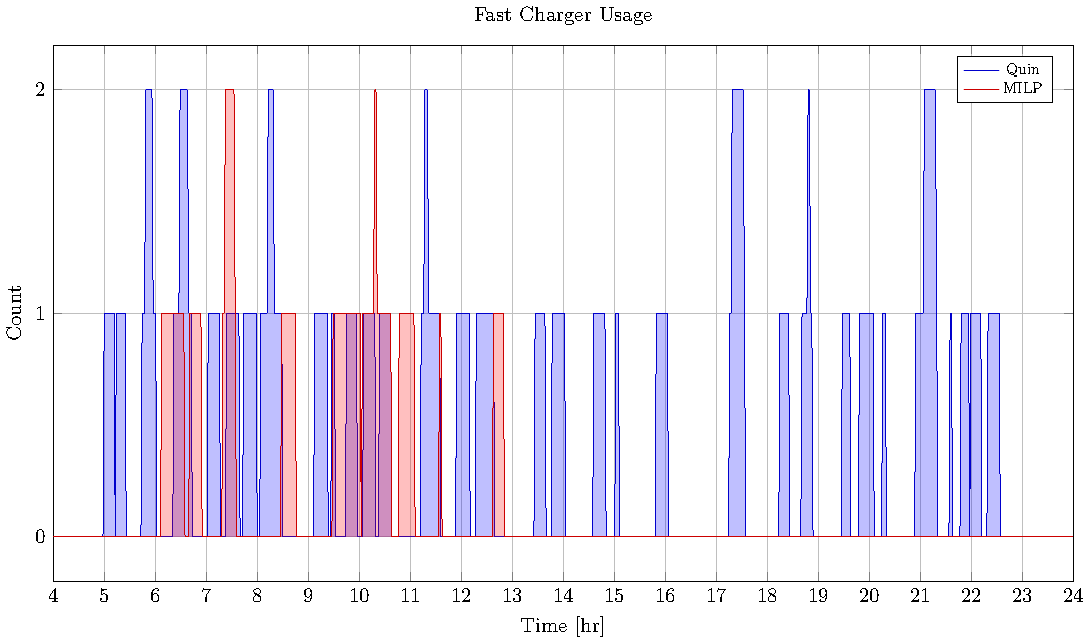
\includegraphics[width=0.6\textwidth]{img/sa-pap-paper-bad/charger-count-fast-milp-qin}
\end{figure}
\begin{figure}[htpb]
\centering
    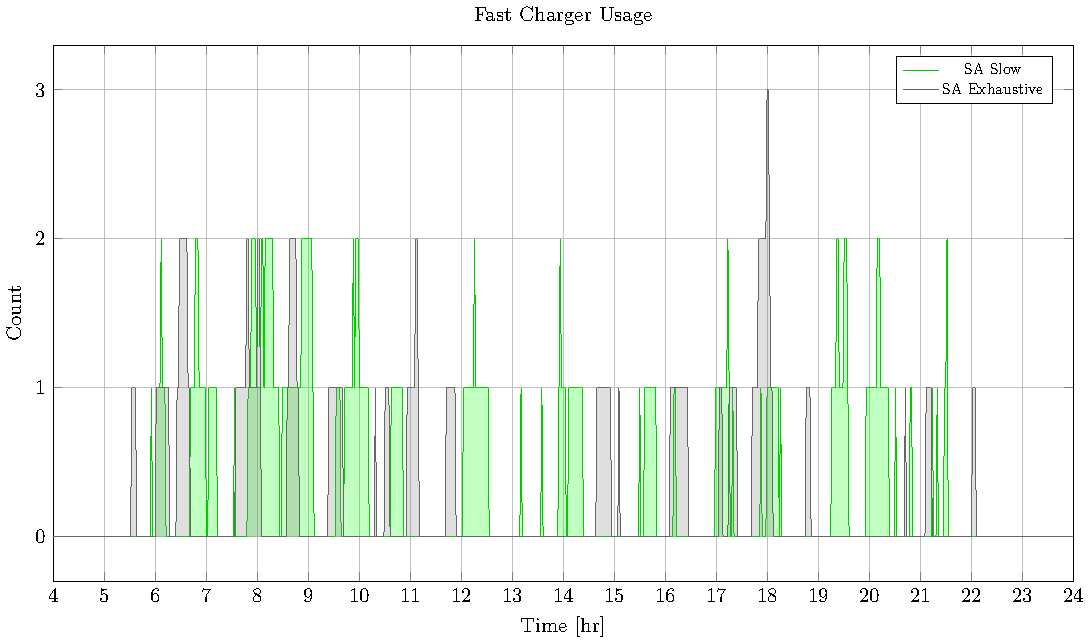
\includegraphics[width=0.6\textwidth]{img/sa-pap-paper-bad/charger-count-fast-sa}
\end{figure}
\end{frame}

\begin{frame}[label={sec:org377c964}]{Power - What Is In The Thesis}
\begin{figure}[htpb]
\centering
    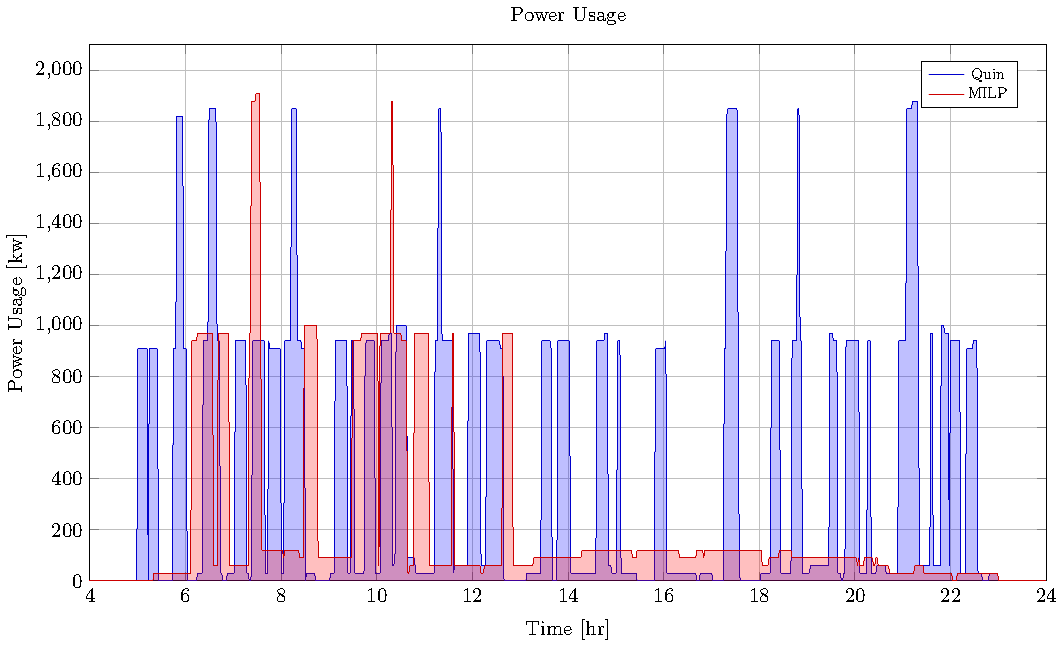
\includegraphics[width=0.6\textwidth]{img/sa-pap-paper-bad/power-milp-qin}
\end{figure}
\begin{figure}[htpb]
\centering
    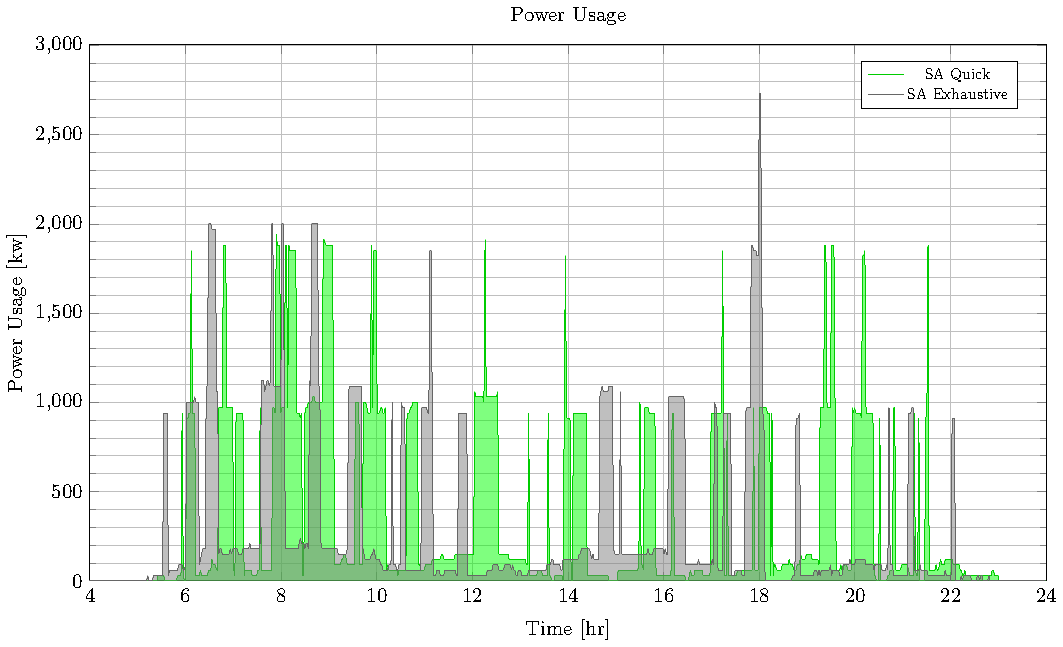
\includegraphics[width=0.6\textwidth]{img/sa-pap-paper-bad/power-sa}
\end{figure}
\end{frame}
\begin{frame}[label={sec:orge33128d}]{Energy - What Is In The Thesis}
\begin{figure}[htpb]
\centering
    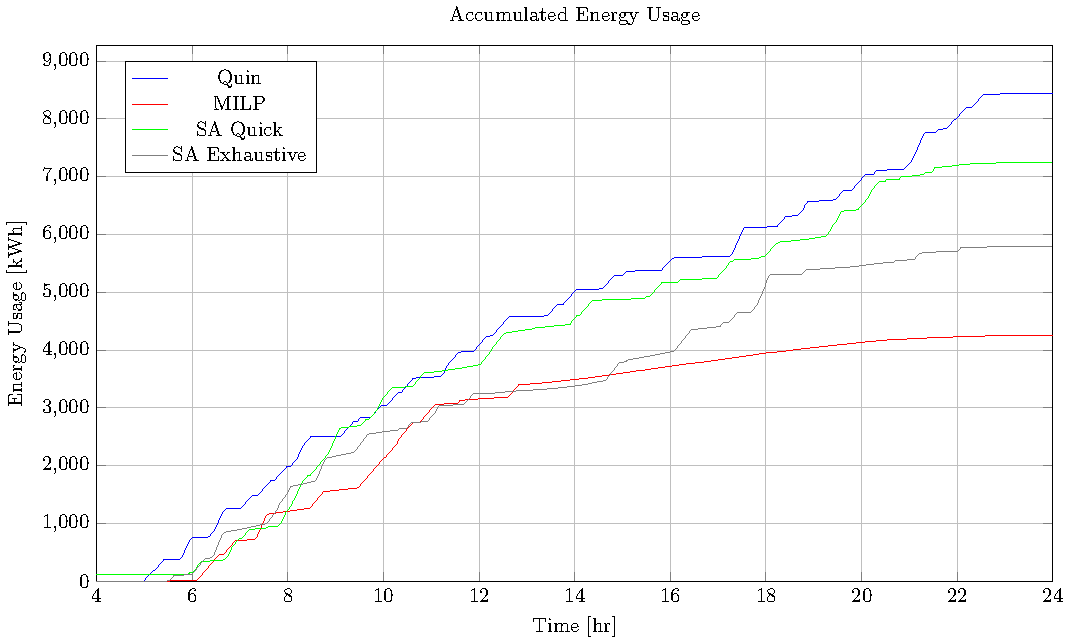
\includegraphics[width=0.6\textwidth]{img/sa-pap-paper-bad/energy}
\end{figure}
\end{frame}

\begin{frame}[label={sec:org1ea1eb2}]{What Happened?}
\begin{figure}[htpb]
\centering
    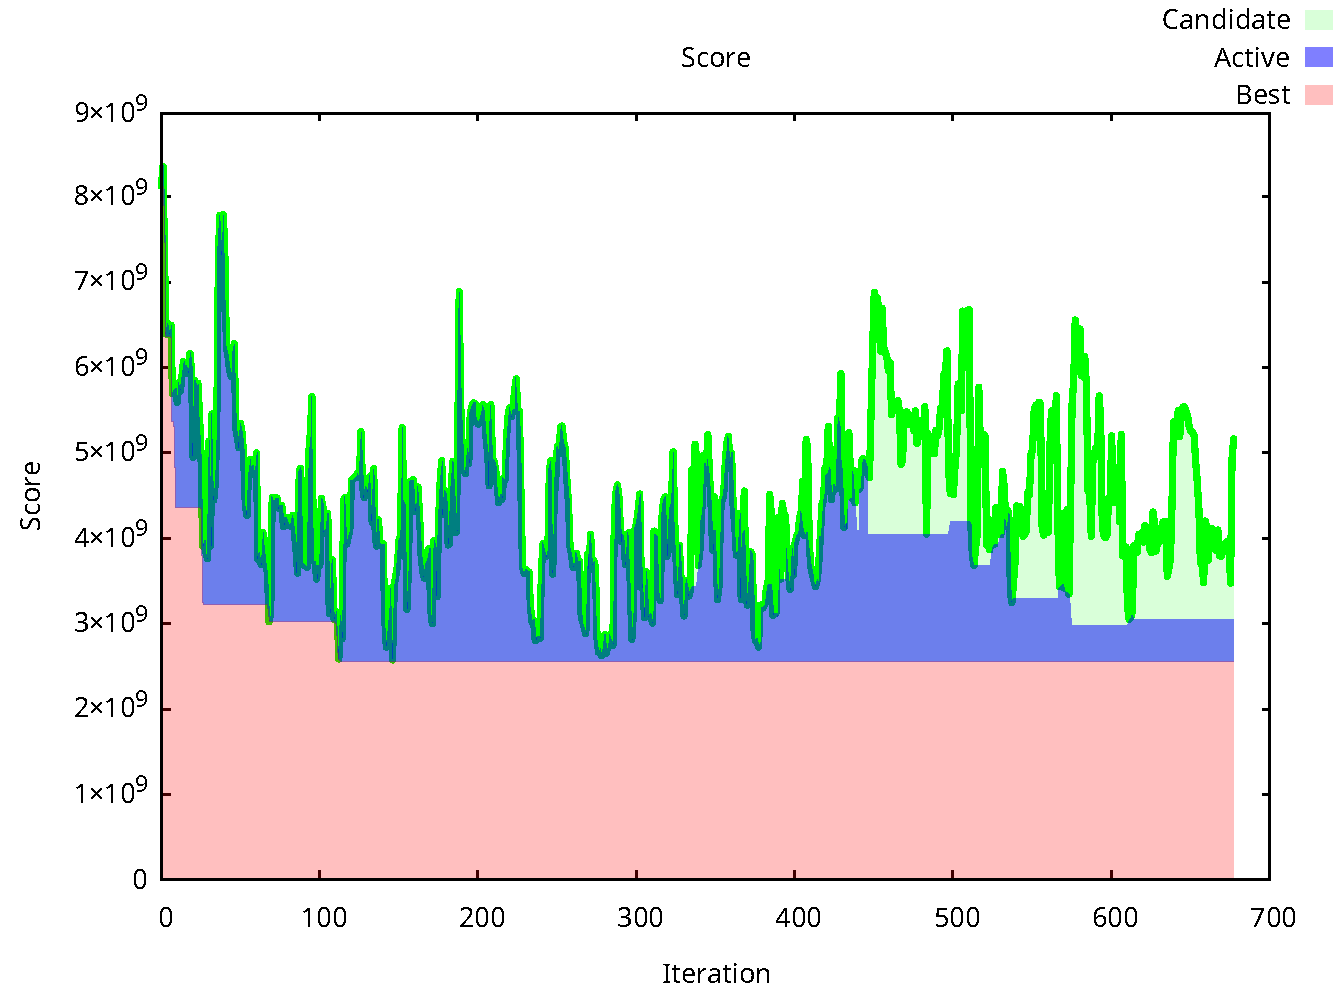
\includegraphics[width=0.6\textwidth]{img/score-diverge}
\end{figure}

\begin{itemize}
\item Candidate solutions diverge
\item Hard time handling ``difficult'' routes
\end{itemize}
\end{frame}
\begin{frame}[label={sec:orgf5abf08}]{How To Resolve This Problem?}
\begin{figure}[htpb]
\centering
    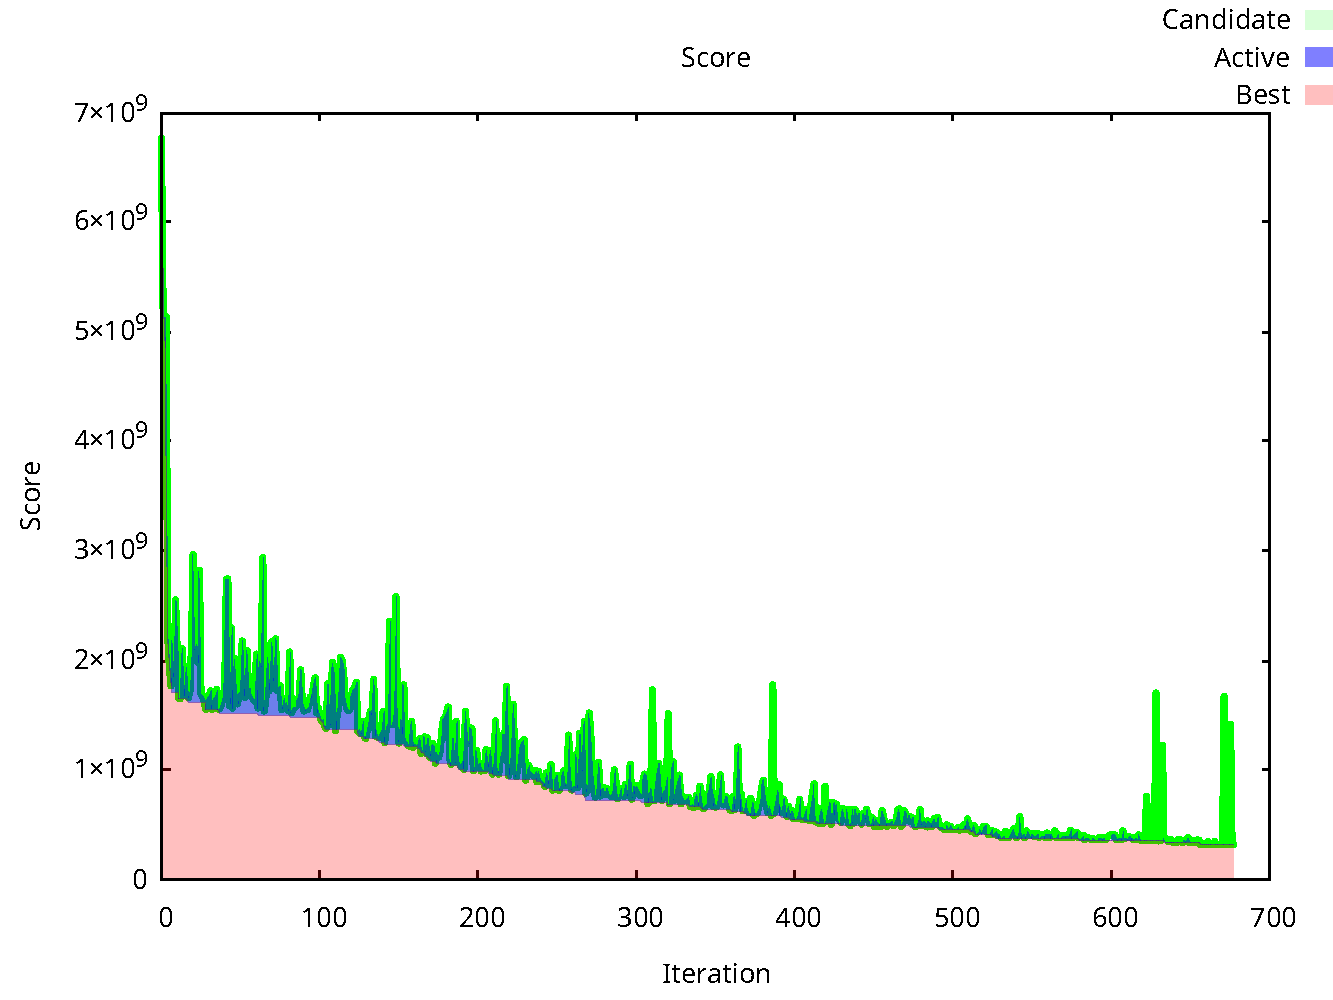
\includegraphics[width=0.6\textwidth]{img/score-convergence}
\end{figure}

\begin{itemize}
\item Reverse search and weight the visit indices
\item Be more aggressive in exploiting the best solution
\end{itemize}
\end{frame}

\begin{frame}[label={sec:org1702709}]{Score Convergence Comparison}
\begin{columns}
\begin{column}{0.5\columnwidth}
\begin{center}
Before Fix
\end{center}

\begin{figure}[htpb]
\centering
    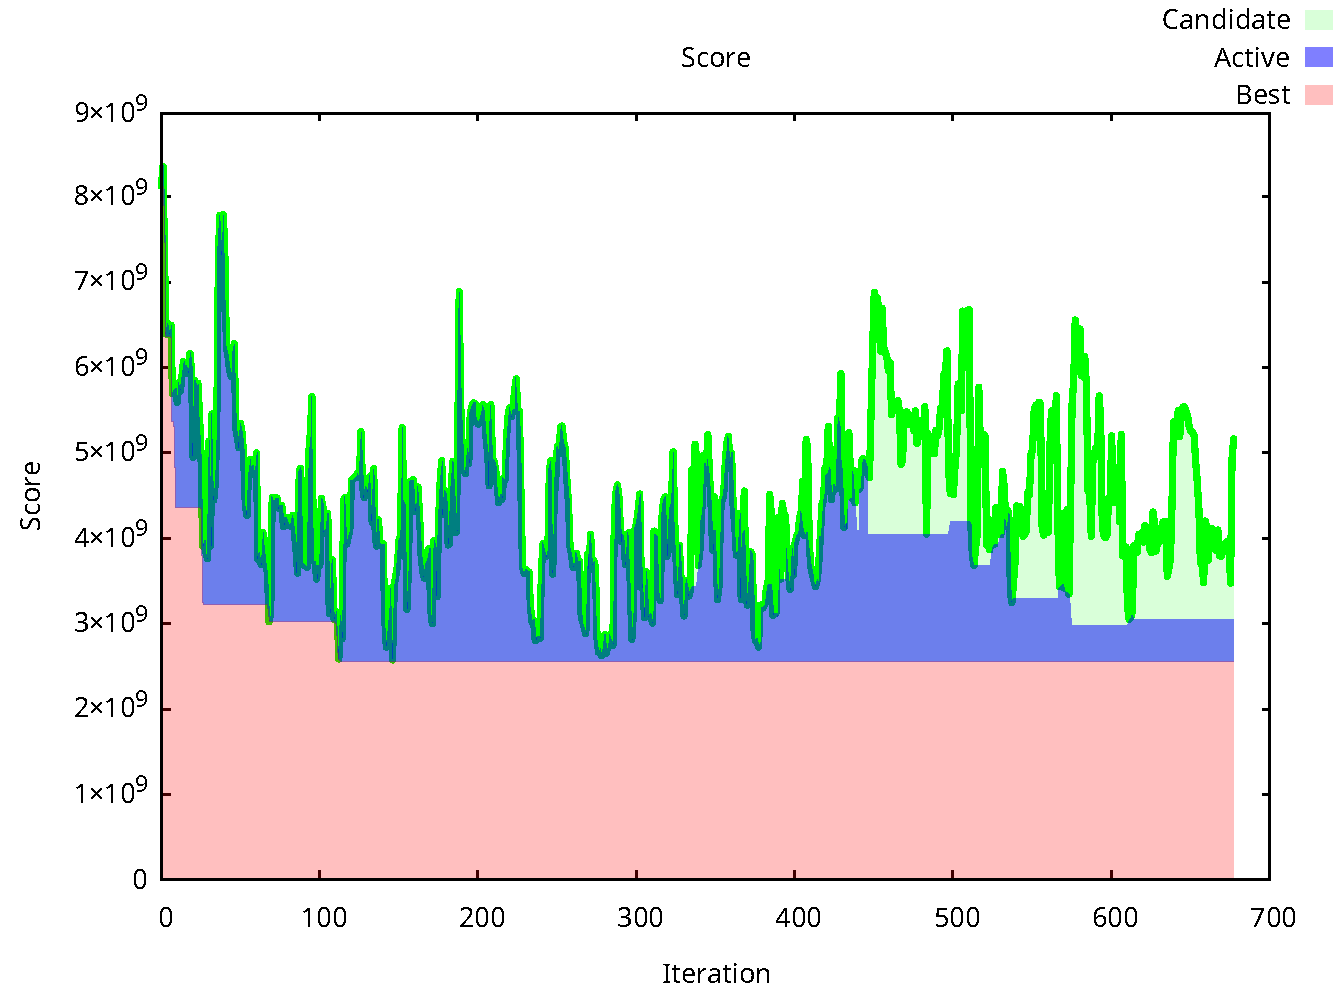
\includegraphics[width=\textwidth]{img/score-diverge}
\end{figure}
\end{column}

\begin{column}{0.5\columnwidth}
\begin{center}
After Fix
\end{center}

\begin{figure}[htpb]
\centering
    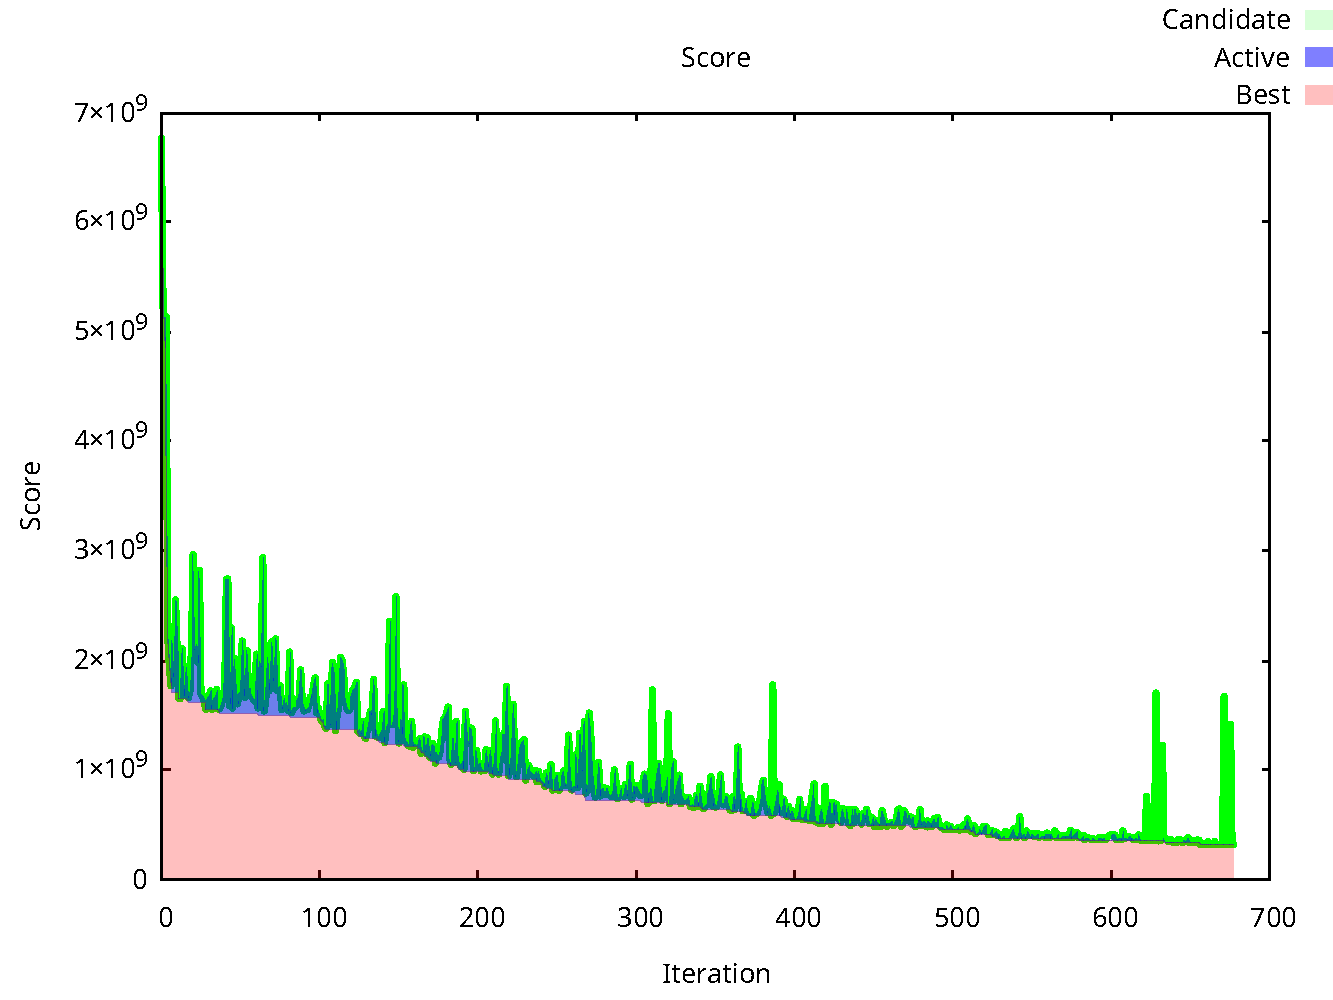
\includegraphics[width=\textwidth]{img/score-convergence}
\end{figure}
\end{column}
\end{columns}
\end{frame}

\begin{frame}[label={sec:orgc5978d5}]{Results - What Is Not In The Thesis}
\begin{center}
\begin{tabular}{lrr}
\alert{Model} & \alert{Execution Time} [s] & \alert{Iteration} [s]\\[0pt]
\hline
MILP & 1900 & N/A\\[0pt]
Quick & 1532.8 & 0.4\\[0pt]
Heuristic & 1916 & 0.5\\[0pt]
\end{tabular}
\end{center}

\begin{columns}
\begin{column}{0.5\columnwidth}
\begin{itemize}
\item \(T_0 = 90000\)
\item \(\beta = 0.997\)
\end{itemize}
\end{column}
\begin{column}{0.5\columnwidth}
\begin{itemize}
\item \(|t| = 3797\)
\item \(n_K = 500\)
\end{itemize}
\end{column}
\end{columns}
\end{frame}

\begin{frame}[label={sec:org5bfd931}]{Schedule - What Is Not In The Thesis}
\begin{figure}[htpb]
\centering
    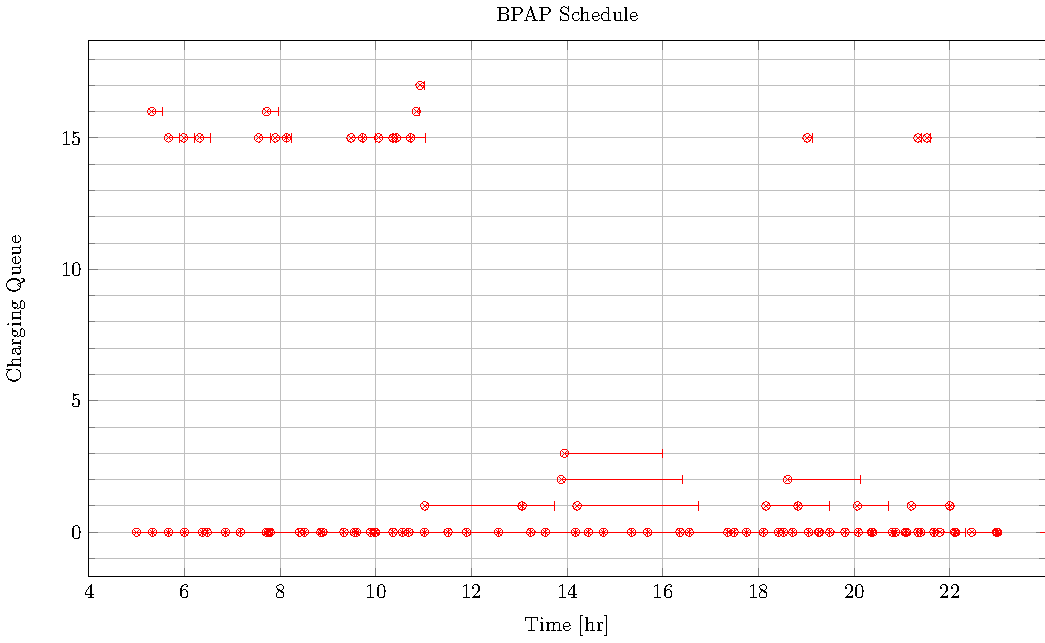
\includegraphics[width=0.75\textwidth]{img/sa-pap-paper-good/schedule-milp}
\end{subfigure}
\begin{subfigure}[t]{\textwidth}
\centering
    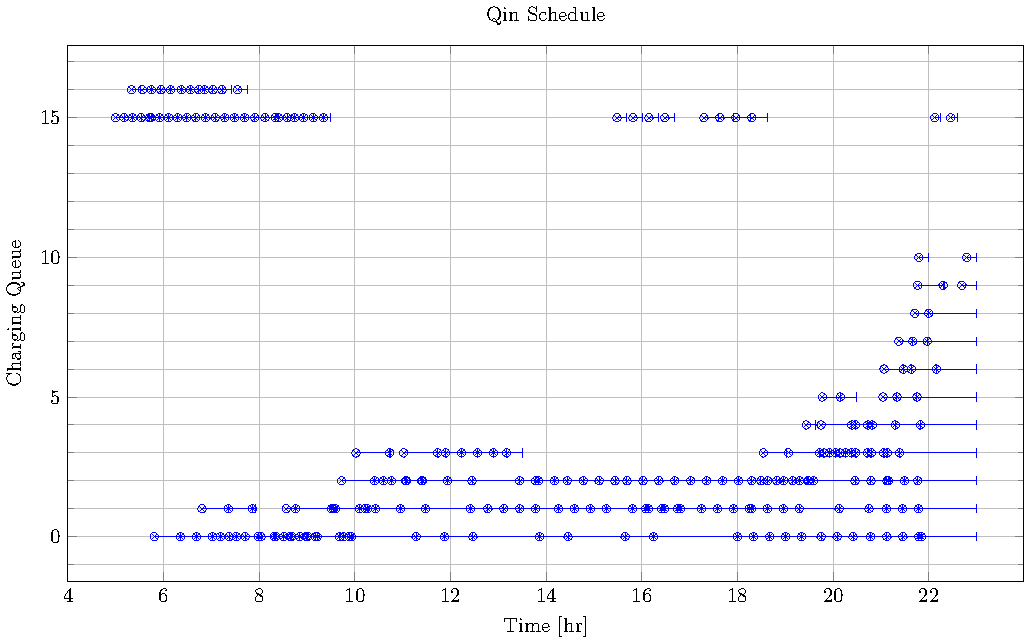
\includegraphics[width=0.75\textwidth]{img/sa-pap-paper-good/schedule-quinn}
\end{subfigure}
\end{figure}
\end{column}

\begin{column}{0.5\columnwidth}
{\scriptsize
\begin{itemize}
\item Point 3
\item Point 4
\end{itemize}
}

\begin{figure}
\begin{subfigure}[t]{\textwidth}
\centering
    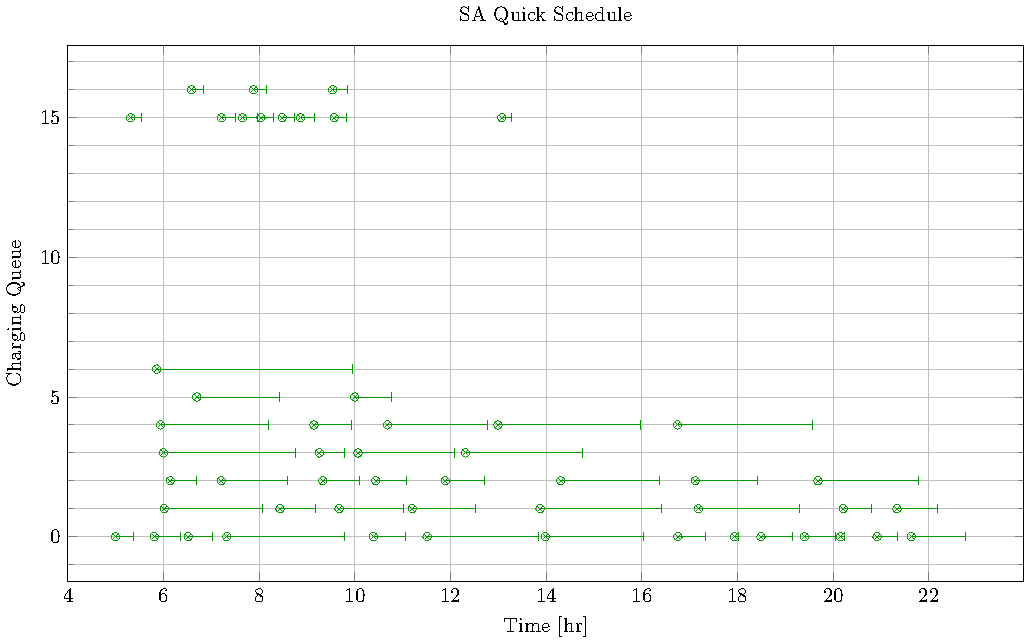
\includegraphics[width=0.75\textwidth]{img/sa-pap-paper-good/schedule-sa-quick}
\end{subfigure}
\begin{subfigure}[t]{\textwidth}
\centering
    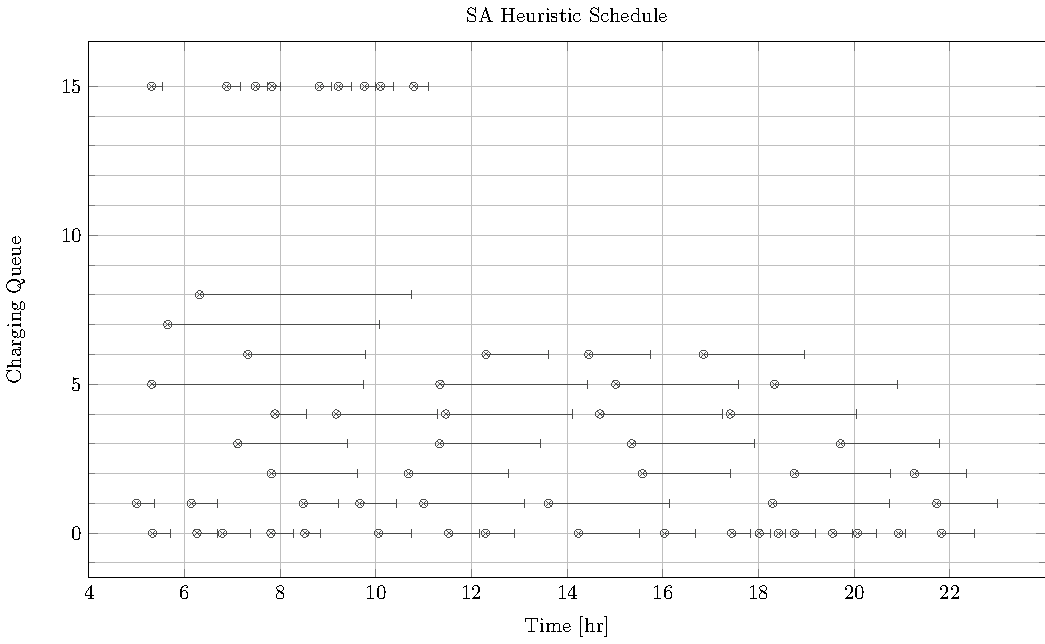
\includegraphics[width=0.75\textwidth]{img/sa-pap-paper-good/schedule-sa-heuristic}
\end{subfigure}
\end{figure}
\end{column}
\end{columns}
\end{frame}

\begin{frame}[label={sec:org539d28c}]{Schedule - What Is Not In The Thesis}
\begin{figure}[htpb]
\centering
    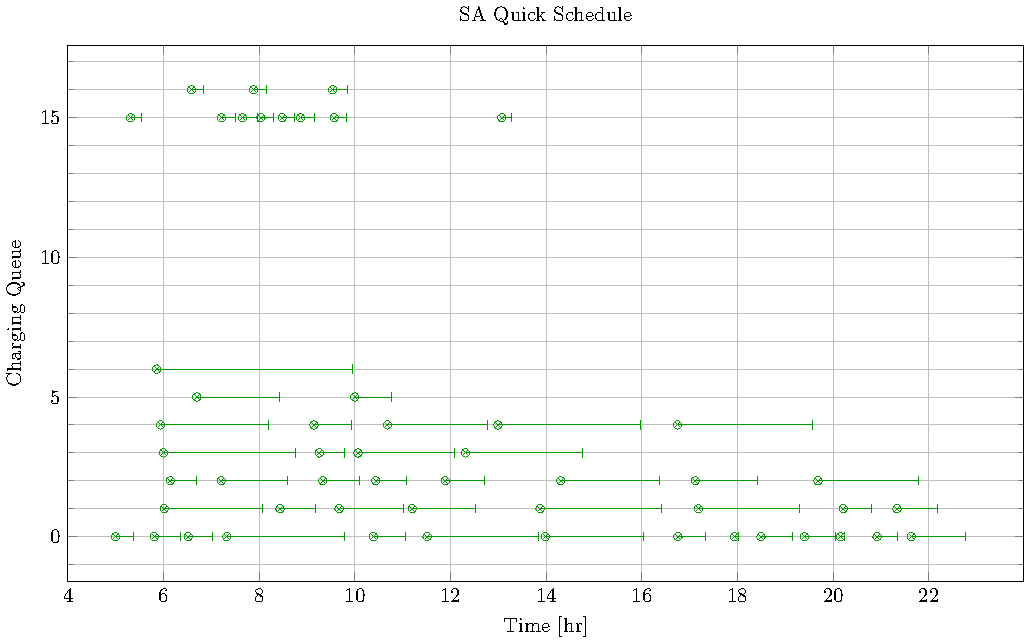
\includegraphics[width=0.6\textwidth]{img/sa-pap-paper-good/schedule-sa-quick}
\end{figure}
\begin{figure}[htpb]
\centering
    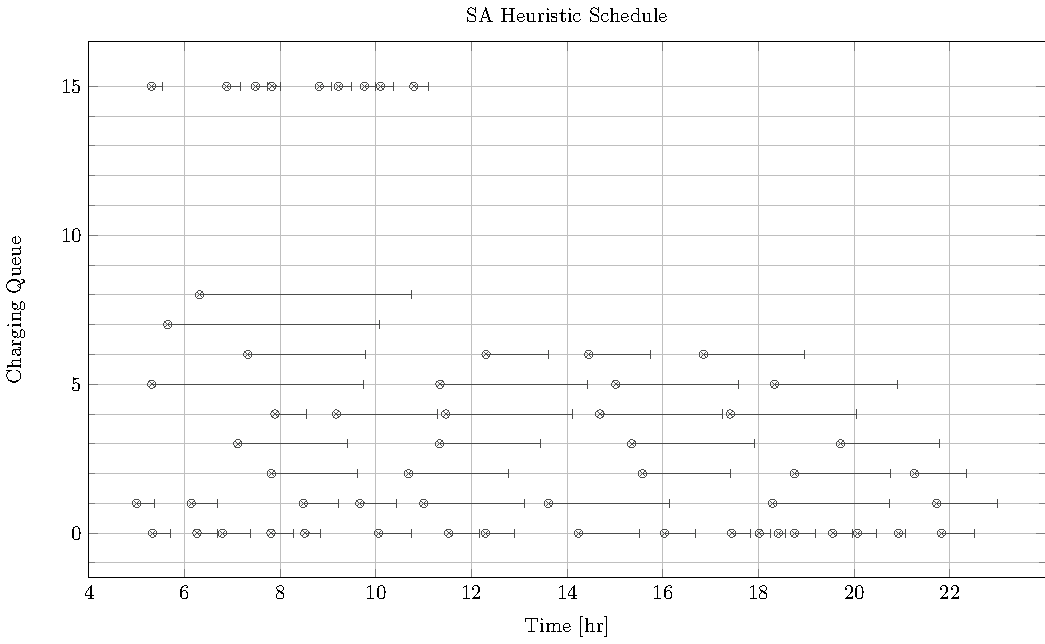
\includegraphics[width=0.6\textwidth]{img/sa-pap-paper-good/schedule-sa-heuristic}
\end{figure}
\end{frame}

\begin{frame}[label={sec:orgc790b73}]{Charger Count - What Is Not In The Thesis}
\begin{figure}[htpb]
\centering
    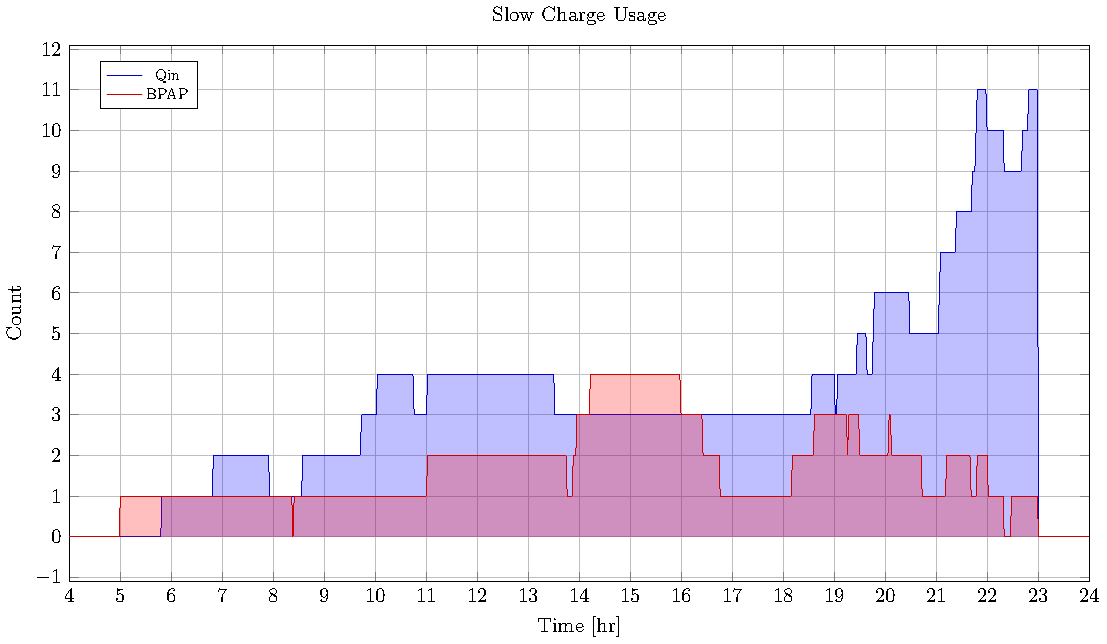
\includegraphics[width=0.6\textwidth]{img/sa-pap-paper-good/charger-count-slow-milp-qin}
\end{figure}
\begin{figure}[htpb]
\centering
    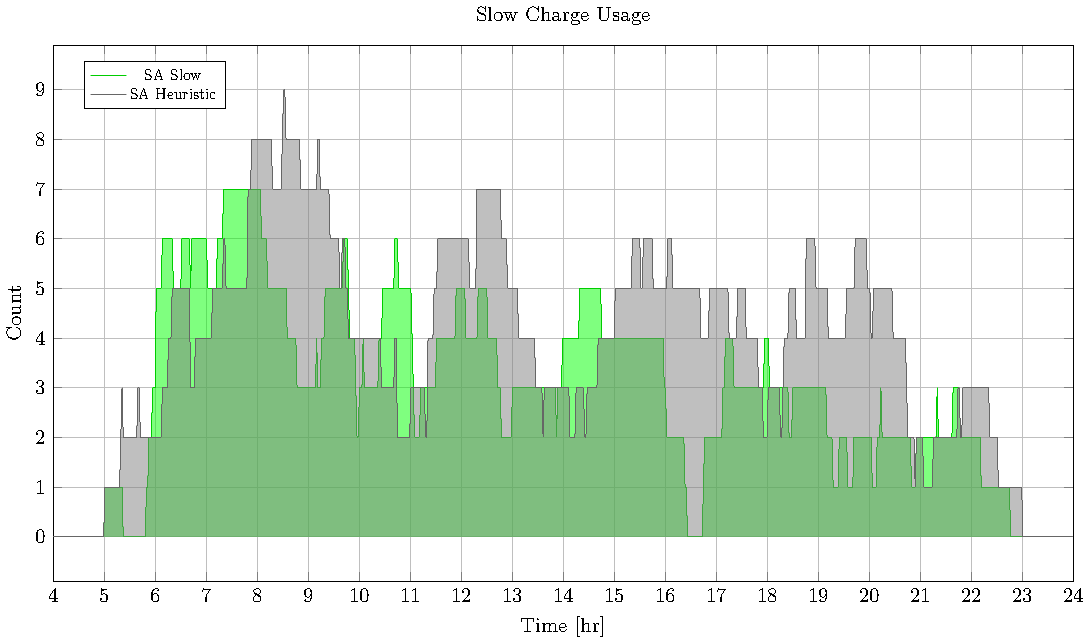
\includegraphics[width=0.6\textwidth]{img/sa-pap-paper-good/charger-count-slow-sa}
\end{figure}
\end{frame}

\begin{frame}[label={sec:orgf6caf70}]{Charger Count - What Is Not In The Thesis}
\begin{figure}[htpb]
\centering
    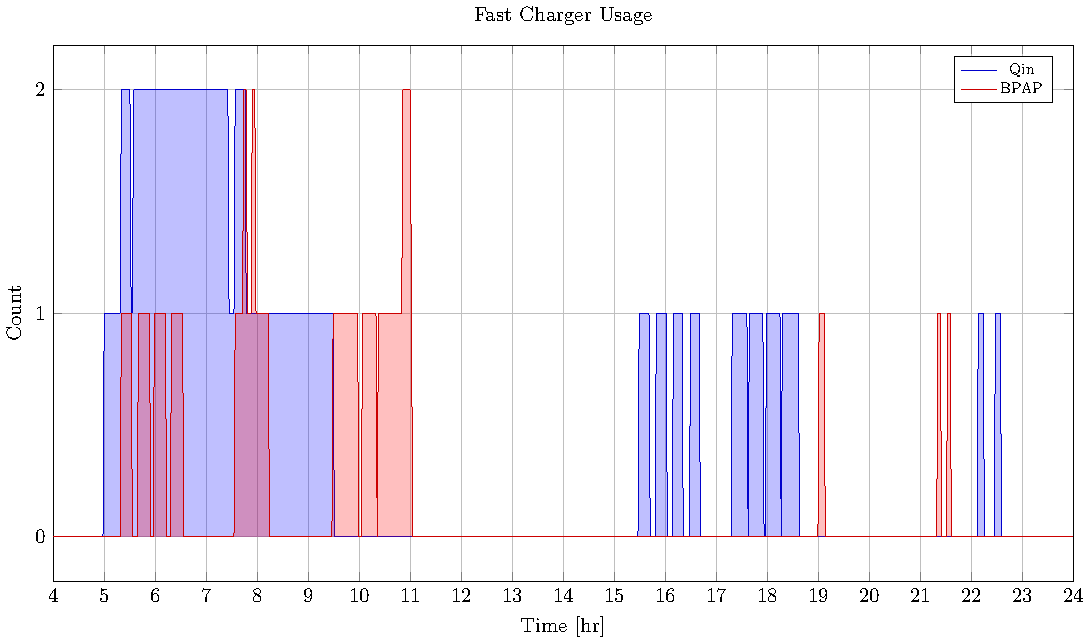
\includegraphics[width=0.6\textwidth]{img/sa-pap-paper-good/charger-count-fast-milp-qin}
\end{figure}
\begin{figure}[htpb]
\centering
    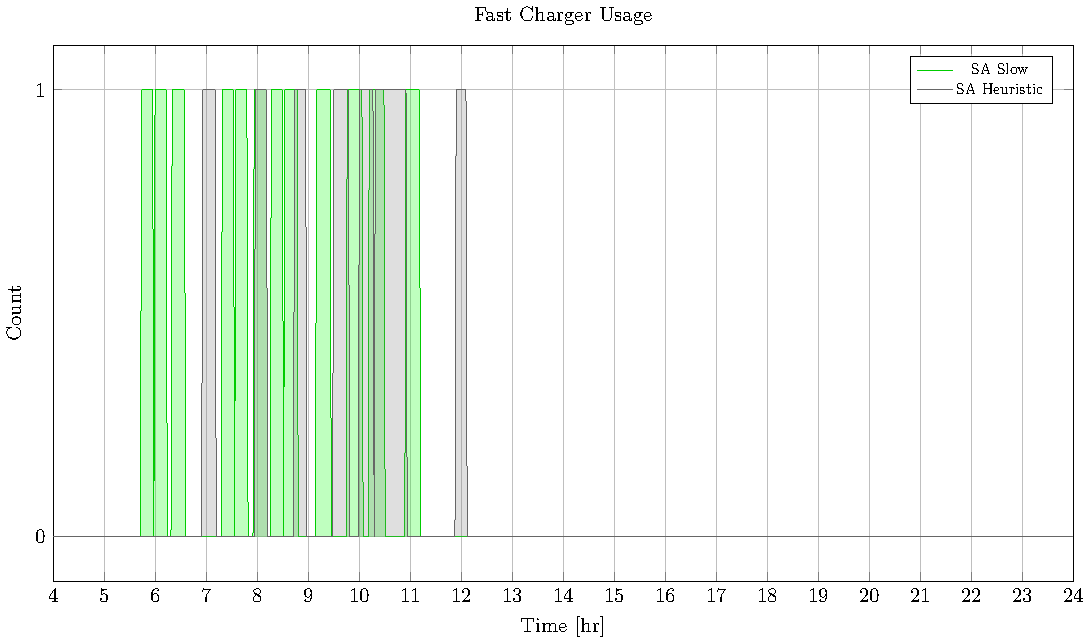
\includegraphics[width=0.6\textwidth]{img/sa-pap-paper-good/charger-count-fast-sa}
\end{figure}
\end{frame}

\begin{frame}[label={sec:orgdf0d78a}]{Power - What Is Not In The Thesis}
\begin{figure}[htpb]
\centering
    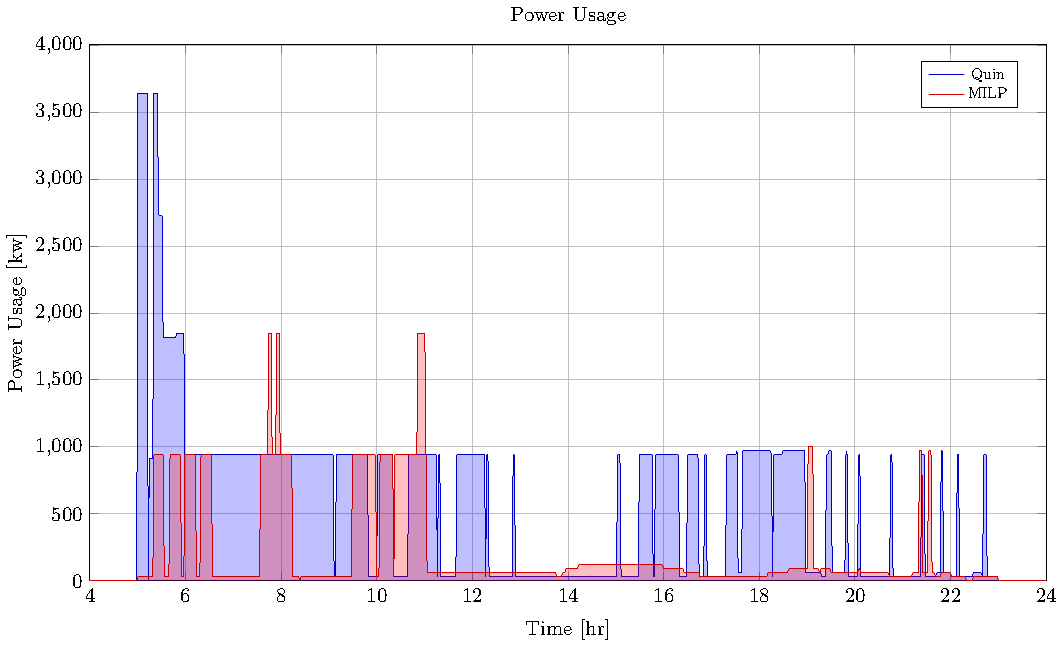
\includegraphics[width=0.6\textwidth]{img/sa-pap-paper-good/power-milp-qin}
\end{figure}
\begin{figure}[htpb]
\centering
    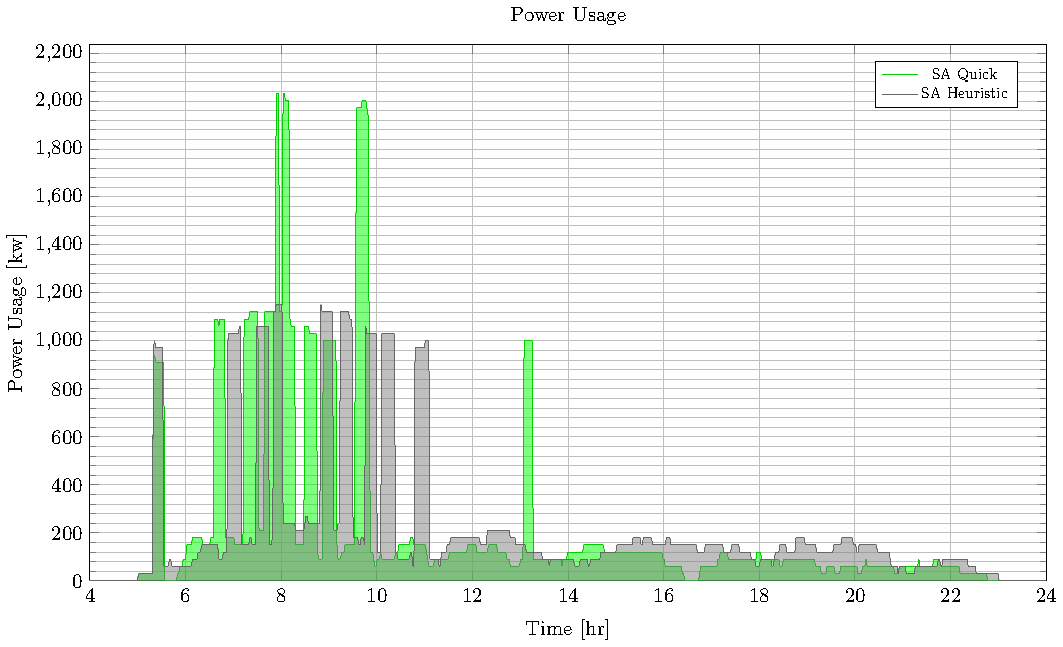
\includegraphics[width=0.6\textwidth]{img/sa-pap-paper-good/power-sa}
\end{figure}
\end{frame}
\begin{frame}[label={sec:orgbd6db57}]{Energy - What Is Not In The Thesis}
\begin{figure}[htpb]
\centering
    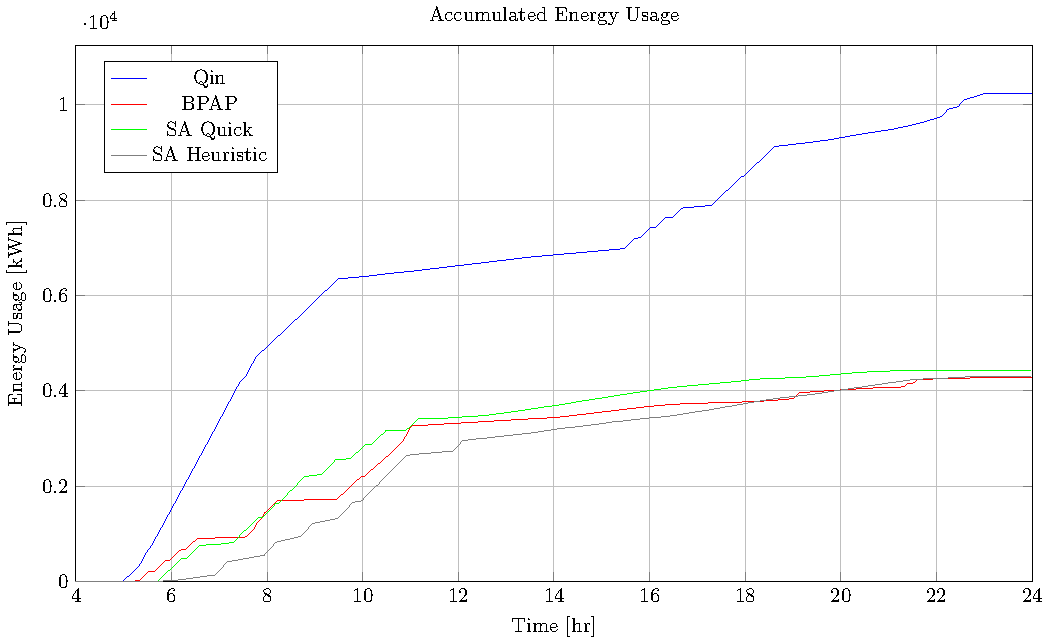
\includegraphics[width=0.6\textwidth]{img/sa-pap-paper-good/energy}
\end{figure}
\end{frame}

\section{The Simulated Annealing Approach With Non-Linear Battery Dynamics}
\label{sec:orgae8c976}
\begin{frame}[label={sec:org9979c1c}]{Introduction}
\begin{itemize}
\item Higher fidelity in approximating charge at high SOC
\item Implemented in SA for simplicity
\end{itemize}
\end{frame}
\begin{frame}[label={sec:orgb0a69c1}]{Non-Linear Battery Dynamics Model}
\begin{itemize}
\item Show function
\item Show plots
\end{itemize}
\end{frame}
\begin{frame}[label={sec:org8991cbb}]{Results}
\begin{itemize}
\item Figures!
\end{itemize}
\end{frame}

\section{Supplemental Slides}
\label{sec:orgaa19478}
\begin{frame}[label={sec:org00ff72f}]{Mixed Integer Linear Programming*}
\begin{align*}
\text{max }        &J = \sum_j c_j x_j + \sum_k d_k y_k&         &               \\
\text{subject to } &\sum_j a_{ij} x_j + \sum_k g_{ik} y_k \le b_i&  &(i = 1,2,...,m)\\
                  &x_j \ge 0&                              &(j = 1,2,...,n)\\
                  &y_k \in \mathbb{Z^+}&                   &(k = 1,2,...,n)\\
\end{align*}

\begin{itemize}
\item \(J\): Objective function
\item \(x_j \in \mathbb{R}\) and \(y_k \in \mathbb{Z}^+\): Decision Variables
\item \(c_j, d_k, a_{ij}, g_{ik}, b_i \in \mathbb{R}\): Parameters
\end{itemize}
\end{frame}


\begin{frame}[label={sec:org7739c71}]{New Visit*}
\begin{algorithm}[H]
  \scriptsize
  \caption{New visit algorithm}
  \label{alg:new-visit}
  \LinesNumbered
  \TitleOfAlgo{New Visit}
  \KwIn{$\Sol$}
  \KwOut{$\bar{\Sol}$}

  \SetKwFunction{Union}{Union}
  \SetKwFunction{findFreeTime}{findFreeTime}

  \Begin
    {
      $i \leftarrow \Sol_{i}$\tcc*{Extract visit index}
      $a \leftarrow \I_{i.a}$\tcc*{Extract the arrivial time for visit $i$}
      $e \leftarrow \I_{i.e}$\tcc*{Extract the departure time for visit $i$}
      $q \leftarrow \I_{i.q}$\tcc*{Extract the current charge queue for visit $i$}
      $\bar{q} \leftarrow \mathcal{U}_{Q}$\tcc*{Select a random charging queue with a uniform distribution}
      $C \leftarrow \mathcal{U}_{\C_q}$\tcc*{Select a random time slice from $\C_q$}

      \If(\tcc*[f]{If there is time available in $C_q^j$}){($\bar{C}, \bar{u}, \bar{d}$) $\leftarrow$ \findFreeTime{$C, i, q, a, e$} $\not\in \varnothing$}
         {
           \Return{($i, (\bar{q},\bar{u},\bar{d}),\bar{C}$)}\tcc*[f]{Return visit}
         }

         \Return{($\varnothing$)}\tcc*{Return nothing}
    }
\end{algorithm}
\end{frame}

\begin{frame}[label={sec:orgf4a3f2a}]{Slide Visit}
\begin{algorithm}[H]
  \scriptsize
  \caption{Slide Visit Algorithm} \label{alg:slide-visit}
  \LinesNumbered
  \TitleOfAlgo{Slide Visit}
  \KwIn{$\Sol$}
  \KwOut{$\bar{\Sol}$}

    \SetKwFunction{Purge}{Purge}

    \Begin
    {
      $(i, \I, \bar{\C}) \leftarrow$\Purge{$\Sol$}\tcc*{Purge visit $i$ from charger availibility matrix}
      $C \leftarrow \bar{C}_{i.q_i}$\tcc*{Get the time availability of the purged visit}

      \tcc{If there is time available in $C$}
      \If{($\bar{C}, \bar{u}, \bar{d}$) $\leftarrow$ \findFreeTime{$C$, $\Sol_i$, $\I_q$, $\I_{i.a}, \I_{i.e}$} $\not\in \varnothing$}
      {
        \Return{($i, \I, (\I_{i.q_i},\bar{u},\bar{d}),\bar{C}$)}\tcc*[f]{Return updated visit}
      }

        \Return{($\varnothing$)}\tcc*{Return nothing}
    }
  \end{algorithm}
\end{frame}

\begin{frame}[label={sec:orgb50f8bb}]{New Charger}
\begin{algorithm}[H]
  \scriptsize
  \caption{New Charger Algorithm} \label{alg:new-charger} \LinesNumbered \TitleOfAlgo{New Charger} \KwIn{$\Sol$}
  \KwOut{$\bar{\Sol}$}

    \SetKwFunction{Purge}{Purge}

    \Begin
    {
      $(i, \I, \bar{\C}) \leftarrow$\Purge{$\Sol$}\tcc*{Purge visit $i$ from charger availibility matrix}
      $q \leftarrow \mathcal{U}_{Q}$\tcc*{Select a random charging queue with a uniform distribution}

      \If(\tcc*[f]{If there is time available in $C_{q}$}){($\bar{C}, \bar{u}, \bar{d}$) $\leftarrow$ \findFreeTime{$\bar{\C}_{i.q}$, $\Sol_i$, $\I_q$, $\I_{i.a}, \I_{i.e}$} $\not\in \varnothing$}
      {
        \tcc{Return visit, note $u$ and $d$ are the original inital/final charge times.}
        \Return{($i, \I, (q,\I_{i.u}, \I_{i.d}),\bar{\C}$)}
      }

      \Return{($\varnothing$)}\tcc*{Return nothing}
    }
  \end{algorithm}
\end{frame}

\begin{frame}[label={sec:org101c46d}]{Wait}
\begin{algorithm}[H]
\scriptsize
\caption{Wait algorithm} \label{alg:wait}
    \LinesNumbered
    \TitleOfAlgo{Wait}
    \KwIn{$\Sol$}
    \KwOut{$\bar{\Sol}$}

    \SetKwFunction{Purge}{Purge}

    \Begin
    {
      $(i, \I, \bar{\C}) \leftarrow$\Purge{$\Sol$}\tcc*{Purge visit $i$ from charger availibility matrix}
      $\bar{\C}'_{\I_{i.\Gamma_i}} \leftarrow \C' \cup \{[\I_{i.a}, \I_{i.e}]\}$\tcc*{Update the charger availability matrix for wait queue $\bar{\C}_{i.q_i}$}
      \Return{$(i, \I, (\I_{i.b}, \I_{i.a}, \I_{i.e}), \bar{\C})$}\tcc*[f]{Return visit}
    }
  \end{algorithm}
\end{frame}

\begin{frame}[label={sec:orgf377ef4}]{New Window}
\begin{algorithm}[H]
  \scriptsize
  \caption{New window algorithm} \label{alg:new-window}
  \LinesNumbered
  \TitleOfAlgo{New Window}
  \KwIn{$\Sol$}
  \KwOut{$\bar{\Sol}$}

  \SetKwFunction{NewVisit}{NewVisit}
  \SetKwFunction{Wait}{Wait}

  \Begin
  {
    $\bar{\Sol} \leftarrow$\Wait{$\Sol$}\tcc*{Assign visit to its respective idle queue}
    \If(\tcc*[f]{Add visit $i$ back in randomly})
       {
         $\bar{\bar{\Sol}} \leftarrow$ \NewVisit{$\bar{\Sol}$} $\not\in \varnothing$
       }
       {
         \Return{$\bar{\bar{\Sol}}$} \tcc*[f]{Return visit}
       }

       \Return{($\varnothing$)}\tcc*{Return nothing}
  }
\end{algorithm}
\end{frame}


\begin{frame}[label={sec:org435bd96}]{Charge Schedule Generation*}
\begin{algorithm}[H]
\scriptsize
\caption{Charge schedule generation algorithm} \label{alg:charge-schedule-generation}
    \LinesNumbered
    \TitleOfAlgo{Candidate Solution Generator}
    \KwIn{$\Sol$}
    \KwOut{$\bar{\Sol}$}

    \SetKwFunction{NewVisit}{NewVisit}

    \Begin
    {
        \tcc{Select an unscheduled BEB visit from a randomly indexed set of visits}
        \ForEach {$\I_i \in \I$}
        {
            ($i, \bar{\I}$, $\bar{\C}$) $\leftarrow$ \NewVisit{($\I_i$, $\I$, $\C$)}\tcc*{Assign the bus to a charger}
        }
            \Return{($0, \bar{\I}$, $\bar{\C}$)}
    }
  \end{algorithm}

\begin{center}
\scalebox{0.65}{
\begin{minipage}{1.5\linewidth}
\begin{algorithm}[H]
\scriptsize
\caption{Perturb schedule algorithm} \label{alg:perturb-schedule}

    \LinesNumbered
    \TitleOfAlgo{Perturb Schedule}
    \KwIn{$\Sol$}
    \KwOut{$\bar{\Sol}$}

    \SetKwFunction{PGF}{PGF}

    \Begin
    {
        $p \leftarrow [false; n_A]$\tcc*{Create vector to track priority routes}
        $y^i \leftarrow [1.0; n_V]$\tcc*{Create weight vector for index selection}
        \tcc{Loop through the visits in reverse order}
        \ForEach{$\I_i \leftarrow \I_{|\I|} \text{ TO } \I_{1}$}
        {
            \tcc{If the current visit is part of a priority route}
            \If{$p_{\I_{i.b}} = true$}{$y^i_{\I_i} = y^i_{\I_{i.\xi}}$\;}
            \tcc{Else if the current visit's SOC does below the allowed threshold}
            \ElseIf{$\I_{i.\eta} \le \nu_{\I_{i.b}} \kappa_{\I_{i.b}}$}{
                $p_{\I_{i.b}} = true$\tcc*{Indicate the current BEB's routes are to be prioritized}
                $y^i_{\I_i} = \kappa_{\I_{i.b}} (\nu_{\I_{i.b}}\kappa_{\I_{i.b}} - \I_{i.\eta})$\tcc*{Calculate the weight of the current visit}
            }
        }
        $\I_i\leftarrow\; \W^{y^i}_{\I}$\tcc*{Select an index with a weighted distribution}
        $i \leftarrow\; \I_i$\tcc*{Extract visit index}
        $y^p \leftarrow [y^p_1, y^p_2, ...]$\tcc*{Define the weight of each primitive generator}
        $PGF \leftarrow\; \W^{y^p}_{[1,n_G]}$\tcc*{Select a generator function with weighted distribution}
        $\bar{\Sol} \leftarrow$ \PGF{($i$, $\I$, $\C$)}\tcc*{Excecute the generator function}
        \Return{($0, \bar{\I}$, $\bar{\C}$)}
    }
\end{algorithm}
\end{minipage}}
\end{center}
\end{frame}


\begin{frame}[label={sec:org45c4322}]{Results - What Is In The Thesis*}
\begin{center}
\begin{tabular}{lrr}
\alert{Model} & \alert{Execution Time} [s] & \alert{Iteration} [s]\\[0pt]
\hline
MILP & 3600 & N/A\\[0pt]
Quick & 2275.25 & 0.25\\[0pt]
Heuristic & 3640.4 & 0.4\\[0pt]
\end{tabular}
\end{center}

\begin{columns}
\begin{column}{0.5\columnwidth}
\begin{itemize}
\item \(T_0 = 99999\)
\item \(\beta = 0.999\)
\end{itemize}
\end{column}
\begin{column}{0.5\columnwidth}
\begin{itemize}
\item \(|t| = 3797\)
\item \(n_K = 500\)
\end{itemize}
\end{column}
\end{columns}
\end{frame}

\begin{frame}[label={sec:org58e1190}]{Schedule- What Is In The Thesis}
\begin{figure}[htpb]
\centering
    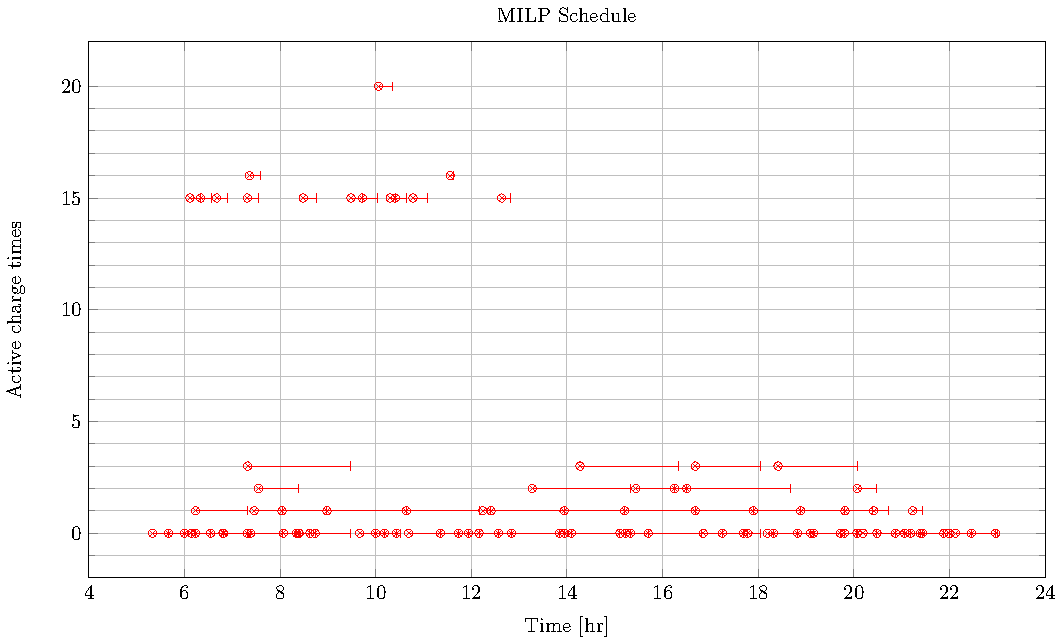
\includegraphics[width=0.6\textwidth]{img/sa-pap-paper-bad/schedule-milp}
\end{figure}
\begin{figure}[htpb]
\centering
    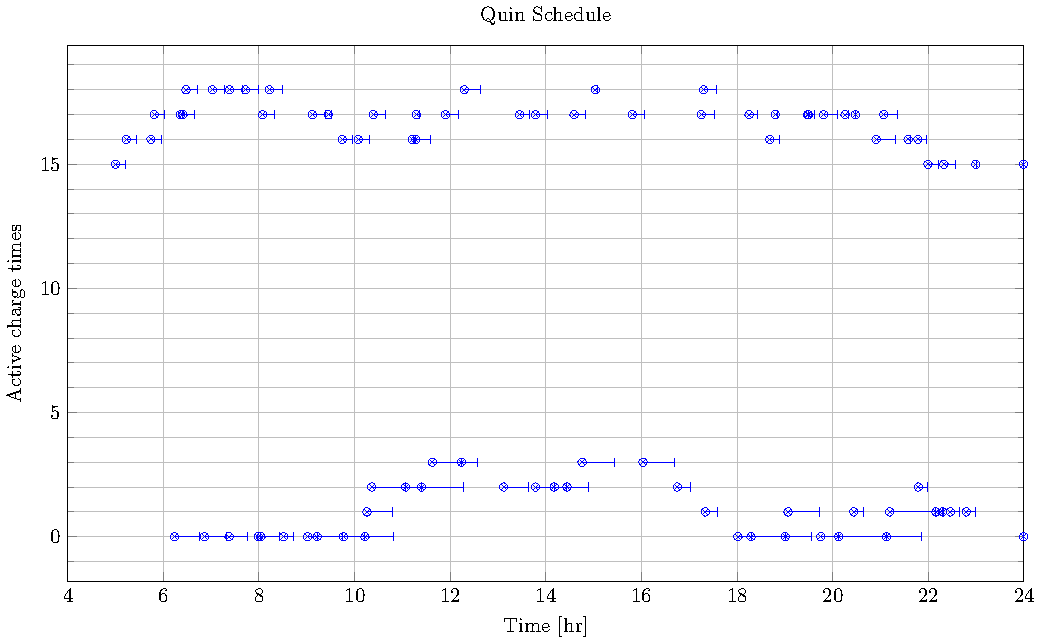
\includegraphics[width=0.6\textwidth]{img/sa-pap-paper-bad/schedule-quinn}
\end{figure}
\end{frame}

\begin{frame}[label={sec:org3f477a6}]{Schedule - What Is In The Thesis}
\begin{figure}[htpb]
\centering
    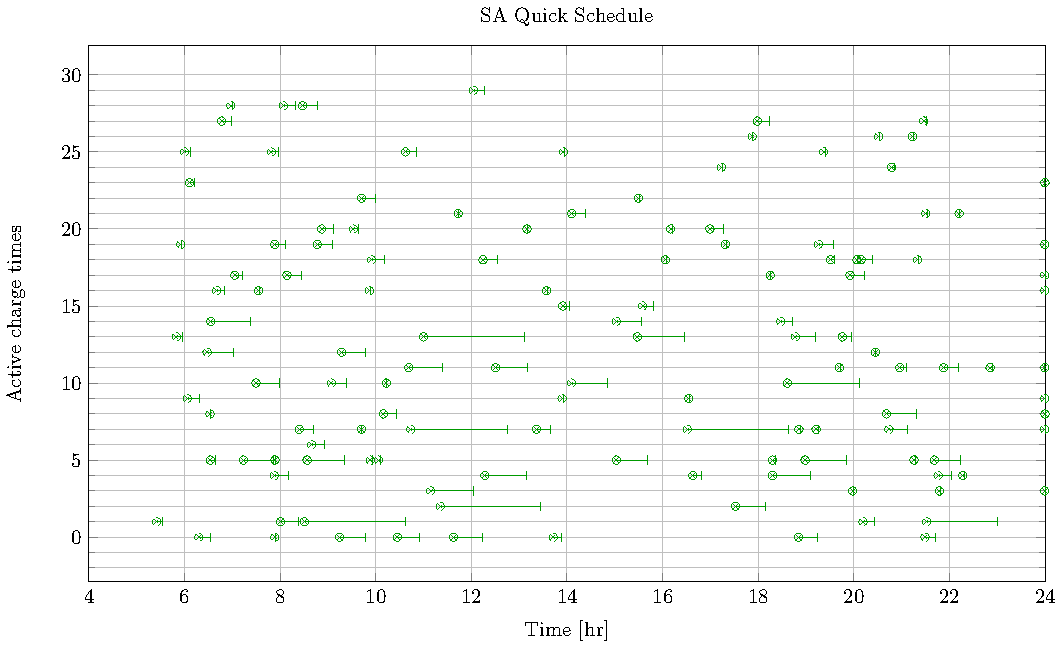
\includegraphics[width=0.6\textwidth]{img/sa-pap-paper-bad/schedule-sa-quick}
\end{figure}
\begin{figure}[htpb]
\centering
    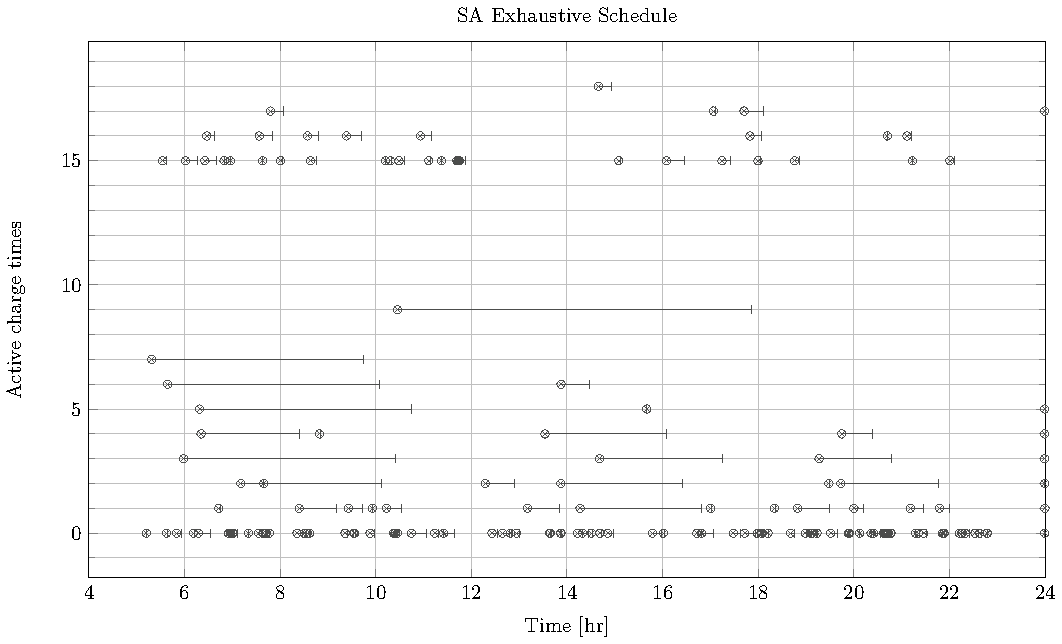
\includegraphics[width=0.6\textwidth]{img/sa-pap-paper-bad/schedule-sa-heuristic}
\end{figure}
\end{frame}

\begin{frame}[label={sec:orgd667ecb}]{Charger Count - What Is In The Thesis}
\begin{figure}[htpb]
\centering
    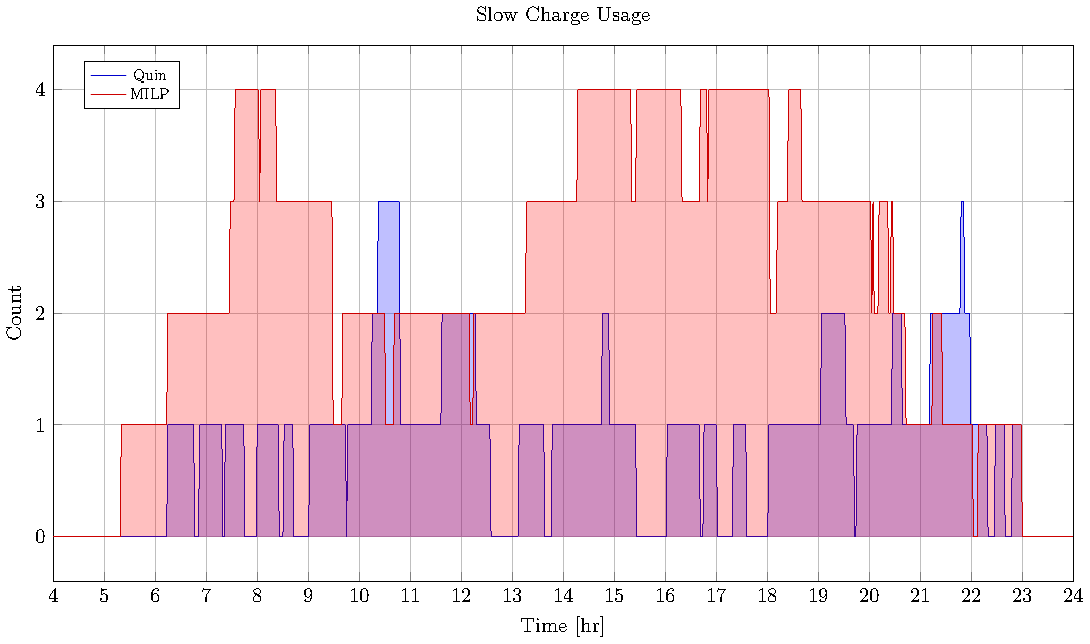
\includegraphics[width=0.6\textwidth]{img/sa-pap-paper-bad/charger-count-slow-milp-qin}
\end{figure}
\begin{figure}[htpb]
\centering
    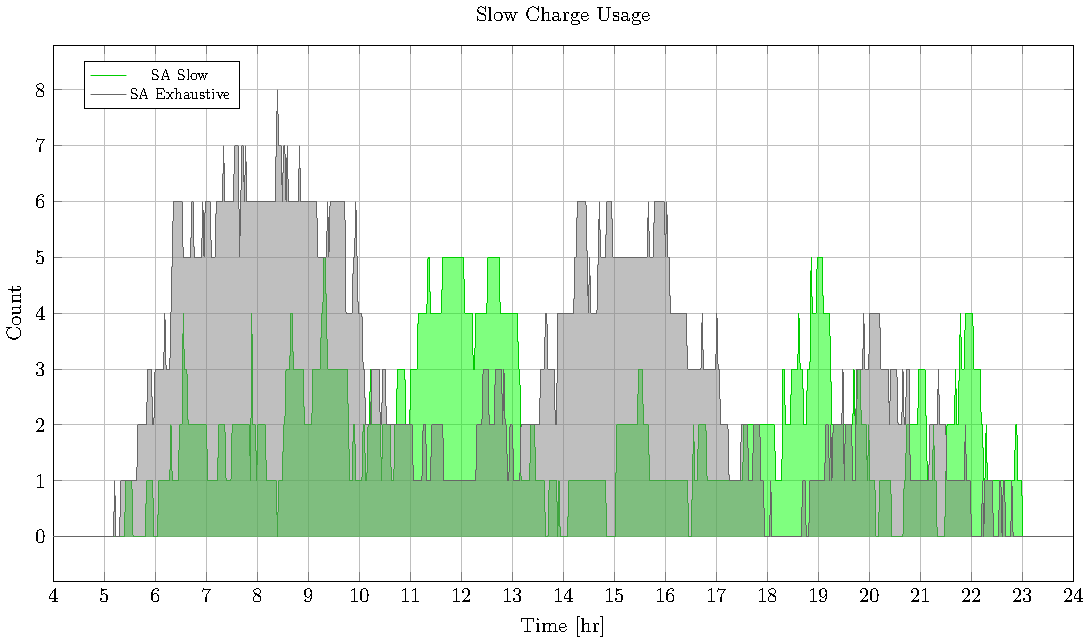
\includegraphics[width=0.6\textwidth]{img/sa-pap-paper-bad/charger-count-slow-sa}
\end{figure}
\end{frame}

\begin{frame}[label={sec:org834c67f}]{Charger Count - What Is In The Thesis}
\begin{figure}[htpb]
\centering
    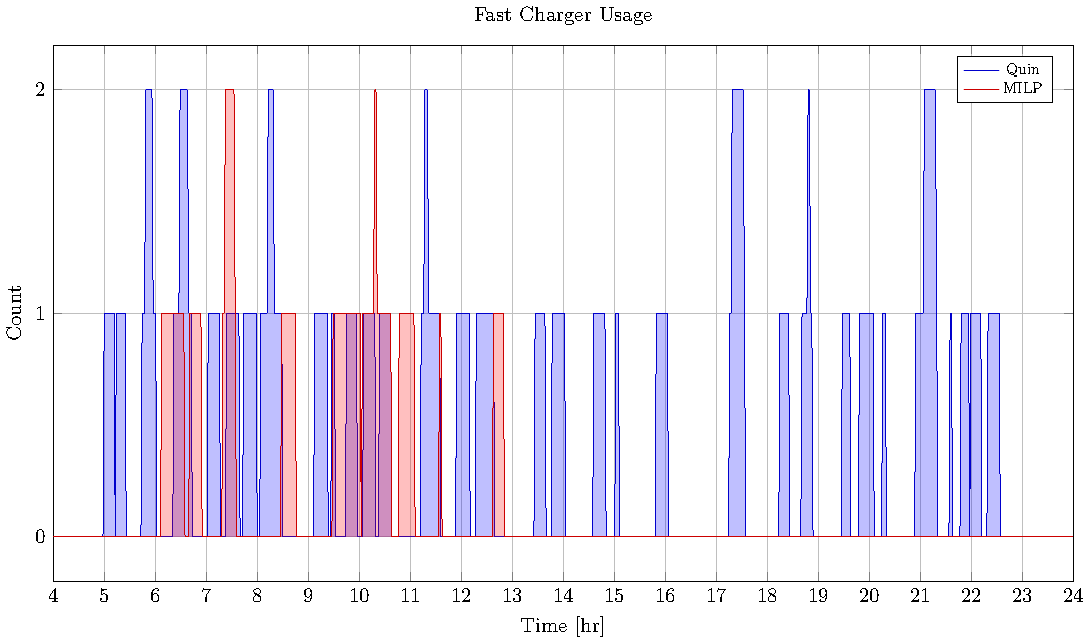
\includegraphics[width=0.6\textwidth]{img/sa-pap-paper-bad/charger-count-fast-milp-qin}
\end{figure}
\begin{figure}[htpb]
\centering
    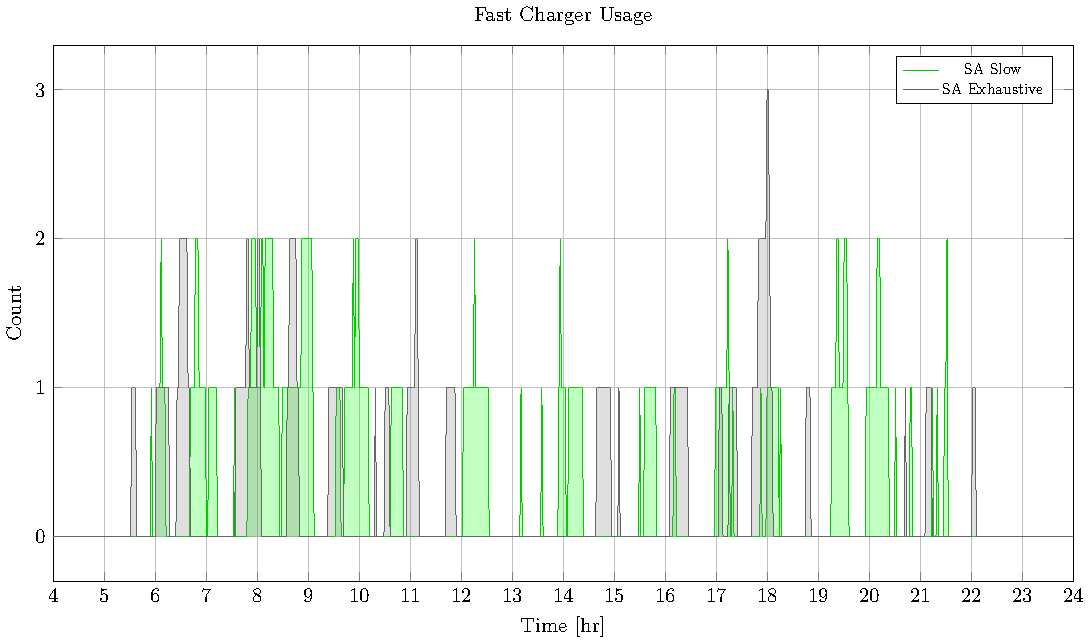
\includegraphics[width=0.6\textwidth]{img/sa-pap-paper-bad/charger-count-fast-sa}
\end{figure}
\end{frame}

\begin{frame}[label={sec:orgda8cd91}]{Power - What Is In The Thesis}
\begin{figure}[htpb]
\centering
    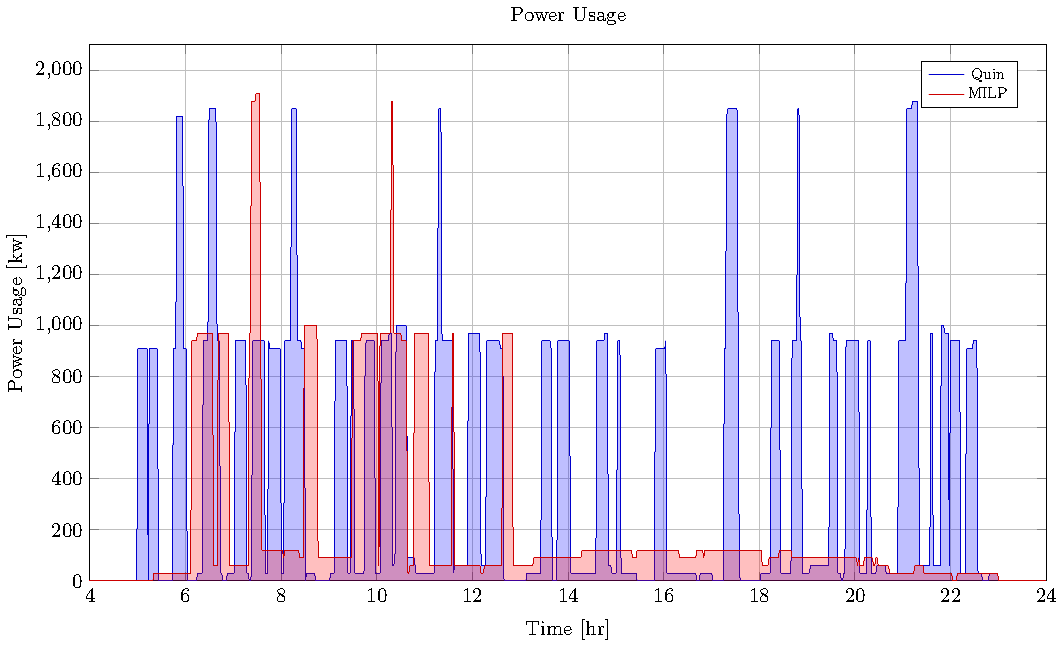
\includegraphics[width=0.6\textwidth]{img/sa-pap-paper-bad/power-milp-qin}
\end{figure}
\begin{figure}[htpb]
\centering
    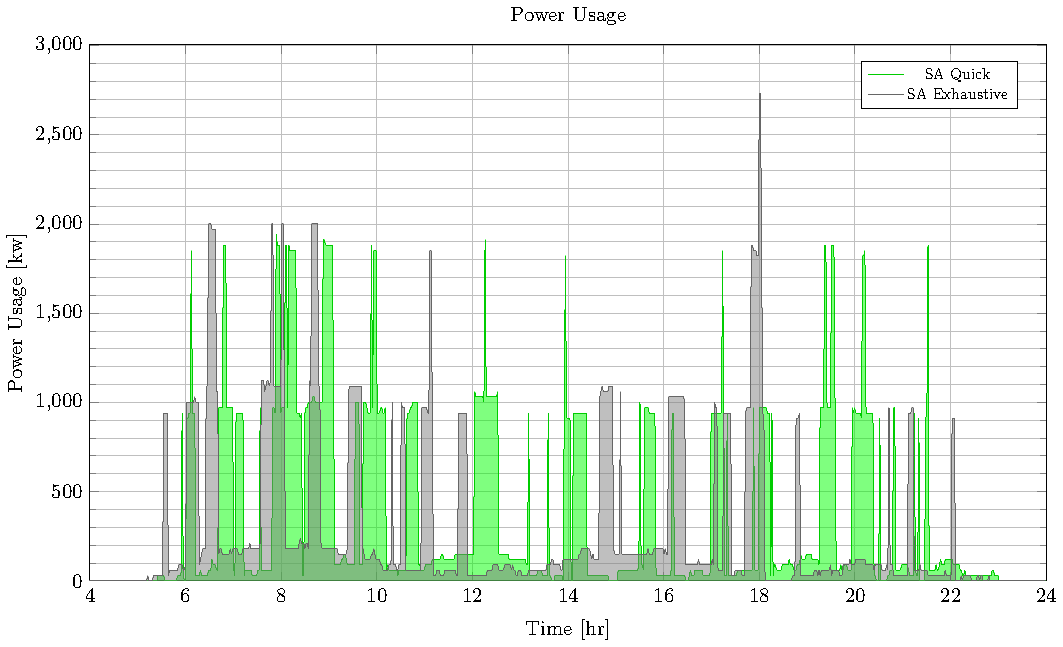
\includegraphics[width=0.6\textwidth]{img/sa-pap-paper-bad/power-sa}
\end{figure}
\end{frame}
\begin{frame}[label={sec:org38002e6}]{Energy - What Is In The Thesis}
\begin{figure}[htpb]
\centering
    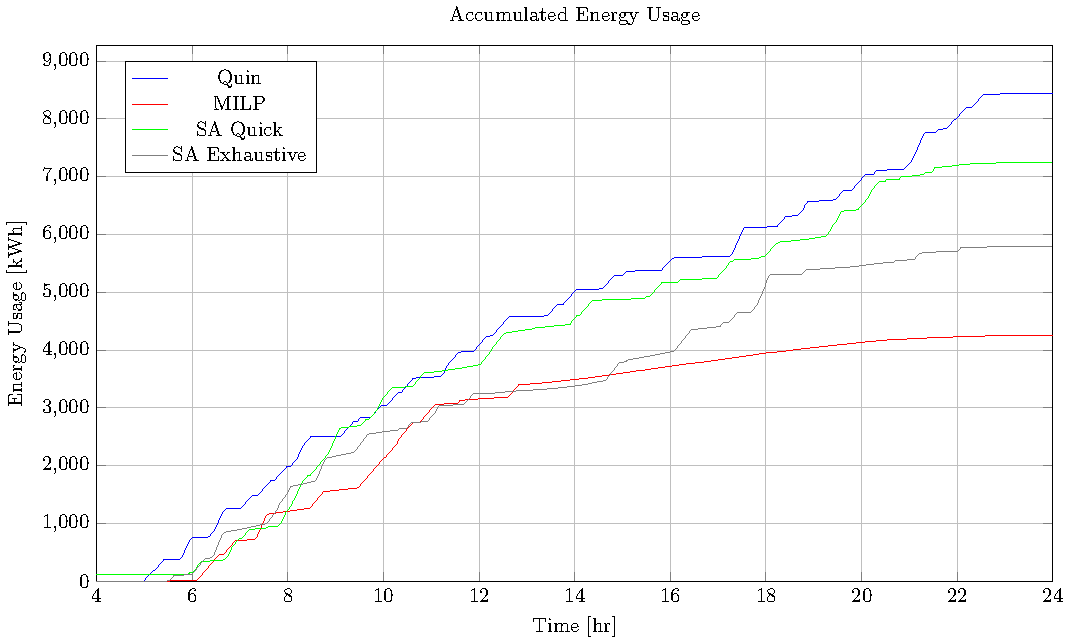
\includegraphics[width=0.6\textwidth]{img/sa-pap-paper-bad/energy}
\end{figure}
\end{frame}

\begin{frame}[label={sec:orgc40313a}]{What Happened?}
\end{frame}
\begin{frame}[label={sec:orgf804da2}]{How To Resolve This Problem?}
\begin{figure}[htpb]
\centering
    \includegraphics[width=0.6\textwidth]{img/score-convergence}
\end{figure}

\begin{itemize}
\item Reverse search and weight the visit indices
\item Be more aggressive in exploiting the best solution
\end{itemize}

\begin{figure}[htpb]
\centering
    \includegraphics[width=0.6\textwidth]{img/score-diverge}
\end{figure}

\begin{itemize}
\item Candidate solutions diverge
\item Hard time handling ``difficult'' routes
\end{itemize}
\end{frame}

\begin{frame}[label={sec:orgcfb7869}]{Score Convergence Comparison}
\begin{columns}
\begin{column}{0.5\columnwidth}
\begin{center}
Before Fix
\end{center}

\begin{figure}[htpb]
\centering
    \includegraphics[width=\textwidth]{img/score-diverge}
\end{figure}
\end{column}

\begin{column}{0.5\columnwidth}
\begin{center}
After Fix
\end{center}

\begin{figure}[htpb]
\centering
    \includegraphics[width=\textwidth]{img/score-convergence}
\end{figure}
\end{column}
\end{columns}
\end{frame}
\end{document}
